\documentclass[11pt,a4paper]{article}

\usepackage{a4wide}
\usepackage{polski}

\usepackage[left=2cm,right=2cm,top=2cm,bottom=2.5cm]{geometry}

\usepackage[utf8]{inputenc}

\usepackage{amsmath}
\usepackage{graphicx}
\usepackage{xcolor}

\usepackage{float}
\usepackage{relsize}
\usepackage{subcaption}
\usepackage{tabularx}

% sans-serif font
\renewcommand{\familydefault}{\sfdefault}

% headers color
\usepackage{sectsty}
\definecolor{lightblue}{HTML}{0040d4}
\sectionfont{\color{lightblue}}
\subsectionfont{\color{lightblue}}
\subsubsectionfont{\color{lightblue}}

\usepackage[colorlinks=true, allcolors=lightblue]{hyperref}

\usepackage[skip=10pt plus1pt, indent=0pt]{parskip}
\usepackage{indentfirst}

\renewcommand{\_}{\char`_}

\begin{document}

\begin{titlepage}
    \centering
    
\includegraphics[width=\textwidth]{images/header.png}

    \vspace{1.5cm}

    \Huge\textbf{ORKESTRO}

    \LARGE\textbf{APLIKACJA DO ZARZĄDZANIA ZESPOŁAMI MUZYCZNYMI I ORKIESTRAMI}

    \vspace{1.5cm}

    \Large \textbf{Dokumentacja projektowa PZSP2} \\
    \vspace{0.5cm}
    WERSJA 5 \\
    \vspace{0.5cm}
    20.01.2024 \\
    Semestr 24Z

    \vfill

    \Large
    Zespół nr 1: \\
    Dominika Boguszewska \\
    Kacper Kowalczyk \\
    Michał Machnikowski \\
    Andrzej Pultyn

    \vspace{2cm}

    \large Mentor zespołu: Klara Borowa

    \large Właściciel tematu: Katarzyna Nałęcz-Charkiewicz
\end{titlepage}

\tableofcontents
\vspace{10pt}
\listoffigures

\newpage

\section{Wprowadzenie}

\subsection{Cel projektu}

Celem projektu jest stworzenie aplikacji ułatwiającej kierownikom grup muzycznych zarządzanie swoimi zespołami, przekazywanie muzykom informacji dotyczących funkcjonowania grupy oraz bezpieczną dystrybucję nut i innych wykorzystywanych plików.

\subsection{Wstępna wizja projektu}

Aplikacja jest stroną internetową, której liderzy grup muzycznych (kierownicy) używają do zarządzania zespołem, w tym między innymi do: tworzenia grup i podgrup, informowania zarządzanej grupy muzyków o nadchodzących próbach i koncertach, dzielenia się z nimi repertuarem i plikami dotyczącymi utworów (np. nutami), czy przekazywania im dodatkowych informacji. W zarządzaniu mogą pomagać im moderatorzy, którzy mają uprawnienia do wysyłania wiadomości. Muzycy korzystają z serwisu, by w jednym miejscu mieć dostęp do wszystkich potrzebnych im informacji, w czym pomagają im zbiorcze zakładki z powiadomieniami i kalendarzem wydarzeń. Przechowywane w serwisie dane to między innymi: składy grup/podgrup i uprawnienia ich członków, wiadomości, wykonywane utwory, podpięte pod nie pliki (i informacje o użytkownikach, którzy mają do nich dostęp), zaplanowane próby i koncerty, czy informacje o użytkownikach (w tym instrumenty, jakimi potrafią się posługiwać).

\section{Metodologia wytwarzania}

Kompozycja naszego zespołu (biorąc pod uwagę naturalne predyspozycje członków wg klasyfikacji Belbina) ma następujący kształt:
\begin{itemize}
    \item role, które spełnia odpowiednia liczba osób: team worker, specialist, finisher, implementer
    \item role, które spełnia nadmiar osób: evaluator, shaper
    \item role, których nie spełnia nikt w zespole: resource investigator, coordinator, plant
\end{itemize}
Z tych danych wynika, że utrudnione jest zaplanowanie projektu (wspólna wersja wizji, koncepcja implementacji, wykorzystywane narzędzia) i koordynacja pracy, ale nie ma przeszkód w kwestii implementacji. Problem zaplanowania projektu został rozwiązany w taki sposób, że jeden z shaperów zajął się sformułowaniem kompletnej wizji projektu, a pozostali członkowie zespołu na bieżąco oceniali przedstawiane elementy i poddawali pod dyskusję zmiany, które chcieliby wprowadzić. W kwestii znajdowania zewnętrznych zasobów jesteśmy zmuszeni zdać się na zdolności, które posiadamy i godzimy się z prawdopodobieństwem przeoczenia niektórych możliwości. Sposób organizacji pracy zostanie opisany w pozostałej części rozdziału.

Projekt będzie wykonywany miejscami podejściem kaskadowym, a miejscami iteracyjnym. Ze względu na specyfikę przedmiotu przed przystąpieniem do implementacji jesteśmy zobowiązani do wytworzenia i przekazania do zatwierdzenia dokumentacji, która ma dogłębnie opisać zakres projektu i dużą część koncepcji na jego wykonanie. Po wykonaniu pracy również przedstawiamy dokumentację uzupełnioną o kolejne elementy. Tryb pracy przy implementacji projektu nie jest narzucony, ale pożądane jest dodawanie kodu kolejno do poszczególnych funkcji. W tych uwarunkowaniach najlepiej jest wykonać początkowe i końcowe etapy projektu kaskadowo, a w etapach projektowania (częściowo), implementacji i testowania po utworzeniu pewnej podstawy będziemy w stanie dodawać kolejne funkcje serwisu w oddzielnych iteracjach.

Możliwości zastosowania różnych metodyk w pracy nad projektem są ograniczone realiami studiowania – członkowie zespołu są zaangażowani w wiele projektów naraz i mogą mieć dodatkowe obowiązki, przez co nie można zakładać systematycznej pracy całego zespołu. Bardziej realistycznym scenariuszem jest to, że w nieokreślonych momentach dana osoba będzie miała możliwość i motywację, by dodać do projektu duży segment funkcjonalności. W organizacji pracy zdecydowaliśmy się inspirować metodyką Scrum i zastosować jej użyteczne dla nas koncepcje w naszych warunkach:
\begin{itemize}
    \item utrzymywany jest niepełny wewnętrzny „backlog produktu” w postaci możliwie zdekomponowanych funkcji lub zmian, które można niezależnie od siebie dodać do projektu w danym stanie
    \item gdy poszczególne osoby mają możliwość pracować nad projektem, rozpoczynają „sprinty”, zobowiązując się wykonać wybrane pozycje z backlogu w najbliższym czasie („backlog sprintu”) i funkcjonując jak jednoosobowy zespół; komunikacja z grupą odbywa się na bieżąco (np. informowanie o problemach lub wykonaniu funkcji) zamiast organizowania spotkań jak w prawdziwym Scrumie
    \item w spotkaniach z interesariuszami przedstawiamy „incrementy” – funkcje zrealizowane od ostatniego spotkania.
\end{itemize}

\section{Analiza wymagań}

Słownik pojęć:
\begin{itemize}
    \item kierownik (grupy muzycznej) – osoba zarządzająca grupą, dodająca wydarzenia, itd.
    \item moderator – członek grupy o uprawnieniach muzyka, który ma dodatkowo możliwość wysyłania wiadomości
    \item muzyk – członek grupy muzycznej bez żadnych dodatkowych uprawnień, jest w stanie tylko dołączać do grup, odczytywać informacje oraz pobierać zasoby (nuty, nagrania)
    \item użytkownik – aktor zbiorczy dla kierownika, moderatora i muzyka.
\end{itemize}

\subsection{Wymagania użytkownika i biznesowe}

Dla uproszczenia treści wymagań możliwości użytkowników domyślnie odnoszą się do grup, których są członkami (zgodnie z wymaganiem ochrony danych)

Wymagania biznesowe:
\begin{enumerate}
    \item Orkiestra potrzebuje aplikacji organizacyjnej, aby umieścić komunikację i zarządzanie zespołami muzycznymi w jednym miejscu.
\end{enumerate}

\vspace{10pt}

Wymagania użytkownika:
\begin{enumerate}
	\item Kierownik będzie mógł tworzyć (pod)grupy użytkowników.
	\item Kierownik będzie mógł zarządzać członkami (pod)grupy.
	\item Kierownik będzie mógł planować wydarzenia dotyczące (pod)grupy (w szczególności próby i koncerty) z listą uczestników i repertuarem.
	\item Kierownik będzie mógł definiować utwory wykonywane przez grupę.
	\item Kierownik będzie mógł udostępniać dla poszczególnych muzyków pliki dotyczące utworu (w szczególności nuty i nagrania) z oznaczeniem instrumentu.
	\item Kierownik będzie mógł wysyłać wiadomości do podzbioru członków (pod)grupy z opcją wysłania kopii na e-mail.
	\item Kierownik będzie mógł edytować dane w (pod)grupie.
	\item Kierownik będzie mógł usuwać dane w (pod)grupie (w szczególności całość (pod)grupy).
	\item Moderator będzie mógł wysyłać wiadomości do podzbioru członków (pod)grupy z opcją wysłania kopii na e-mail.
	\item Użytkownik będzie mógł dołączać do (pod)grup, do których został zaproszony.
	\item Użytkownik będzie mógł przeglądać plan wydarzeń dla jednej i wszystkich (pod)grup.
	\item Użytkownik będzie mógł decydować o synchronizacji kalendarza wydarzeń ze swoim Google Calendar.
	\item Użytkownik będzie mógł przeglądać wiadomości wysłane do niego w jednej i wszystkich (pod)grupach.
	\item Użytkownik będzie mógł przeglądać utwory wykonywane w (pod)grupie z opcją wyszukiwania.
	\item Użytkownik będzie mógł przeglądać listę plików dodanych dla utworu z opcją pobierania tych, do których ma dostęp oraz wyszukiwania.
	\item Użytkownik będzie mógł łatwo dostać się do udostępnionych mu plików dotyczących wydarzenia.
	\item Użytkownik będzie mógł potwierdzać swoją tożsamość za pomocą konta Google.
	\item Użytkownik będzie mógł korzystać z serwisu w językach polskim oraz angielskim, z możliwością przyszłego rozszerzenia dostępności o inne języki.
	\item Użytkownik będzie mógł komfortowo korzystać z serwisu przy dużym obciążeniu.
	\item Użytkownik będzie mógł korzystać z serwisu przy użyciu różnych urządzeń i oprogramowania (uszczegółowione w wymaganiach S32-S35).
	\item Użytkownik będzie mógł bezpiecznie przechowywać dane w serwisie.
\end{enumerate}

\vspace{10pt}

Wymagania systemowe:
\begin{enumerate}
	\item System pozwoli tworzyć grupy użytkowników (z nazwą i opisem).
	\item System pozwoli tworzyć podgrupy (pod)grupy (z nazwą i opisem).
	\item System pozwoli zapraszać użytkowników do (pod)grupy.
	\item System pozwoli ustalać uprawnienia członków (pod)grupy.
	\item System pozwoli definiować wydarzenia dotyczące (pod)grupy, w szczególności próby i koncerty (z nazwą, opisem, datą i miejscem).
	\item System pozwoli ustalać listę uczestników wydarzenia.
	\item System pozwoli definiować utwory wykonywane przez (pod)grupę (z nazwą i opisem).
	\item System pozwoli przypisywać utwory do wydarzenia, na którym będą wykonywane.
	\item System pozwoli dodawać pliki dotyczące utworu.
	\item System pozwoli oznaczać plik nazwami instrumentów i głosów, których dotyczy.
	\item System pozwoli definiować, jacy użytkownicy mają dostęp do pliku.
	\item System pozwoli wysyłać wiadomości do podzbioru członków (pod)grupy.
	\item System pozwoli wysyłać na skrzynki e-mailowe adresatów kopię tworzonej wiadomości.
	\item System pozwoli edytować dane w (pod)grupie.
	\item System pozwoli usuwać dane w (pod)grupie (w szczególności całość (pod)grupy).
	\item System pozwoli dołączać do (pod)grup na podstawie otrzymywanych zaproszeń.
	\item System pozwoli przeglądać wydarzenia zdefiniowane dla (pod)grupy.
	\item System pozwoli przeglądać kalendarz wydarzeń ze wszystkich (pod)grup danego użytkownika.
	\item System pozwoli synchronizować kalendarz wydarzeń z Google Calendar.
	\item System pozwoli przeglądać wiadomości wysłane do danego użytkownika w (pod)grupie.
	\item System pozwoli przeglądać listę wiadomości, które dany użytkownik otrzymał ze wszystkich (pod)grup.
	\item System pozwoli przeglądać utwory wykonywane w (pod)grupie.
	\item System pozwoli wyszukiwać utwory z listy w (pod)grupie (po nazwie, podpiętym koncercie, wykorzystywanym instrumencie).
	\item System pozwoli przeglądać listę plików dodanych dla utworu.
	\item System pozwoli wyszukiwać pliki spośród tych udostępnionych dla konkretnego utworu (po nazwie, wykorzystywanym instrumencie).
	\item System pozwoli pobierać pliki, które zostały udostępnione dla danego użytkownika.
	\item System pozwoli zbiorczo przeglądać udostępnione dla danego użytkownika pliki z utworów dotyczących wydarzenia.
	\item System pozwoli logować się kontem Google.
	\item System pozwoli wybrać język korzystania z serwisu (w szczególności polski i angielski).
	\item System będzie zaprojektowany w sposób umożliwiający dodawanie zasobów sprzętowych, tak by możliwe było jego płynne działanie przy 1000 jednoczesnych użytkowników oraz 10 jednoczesnych, niezależnych grup.
	\item System będzie udokumentowany, w szczególności w kwestiach wdrożenia oraz dodawania zasobów sprzętowych.
	\item System będzie oferował interfejs graficzny zoptymalizowany dla urządzeń mobilnych.
	\item System będzie oferował interfejs graficzny zoptymalizowany dla komputerów PC.
	\item System będzie dostępny na urządzeniach z systemami Windows, Android, Linux i iOS.
	\item System będzie dostępny poprzez przeglądarki Chrome, Safari, Firefox, Edge i Opera.
	\item System będzie weryfikował tożsamość użytkownika i jego uprawnienia przed wykonaniem operacji na danych.
	\item System będzie funkcjonował zgodnie z przepisami RODO.
	\item System będzie tworzył szyfrowane połączenia z użytkownikami.
	\item System będzie wyposażony w zabezpieczenia przed włamaniami.
\end{enumerate}

\subsection{Wymagania funkcjonalne i niefunkcjonalne}

\begin{figure} [H]
    \centering
    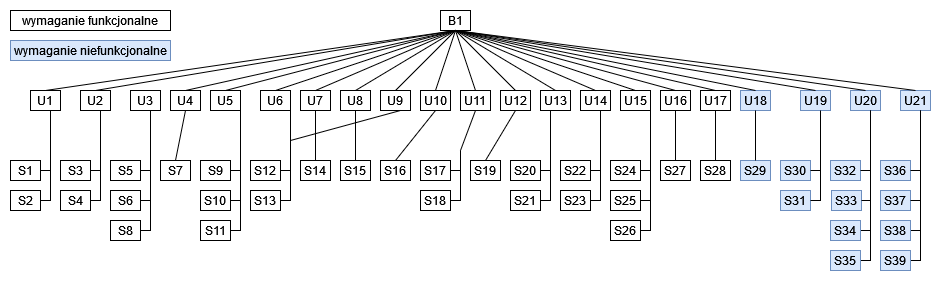
\includegraphics[width=0.95\linewidth]{images/wymagania.png}
    \caption{Diagram powiązań wymagań z podziałem na wymagania funkcjonalne i niefunkcjonalne}
\end{figure}

\subsection{Przypadki użycia}

\begin{figure} [H]
    \centering
    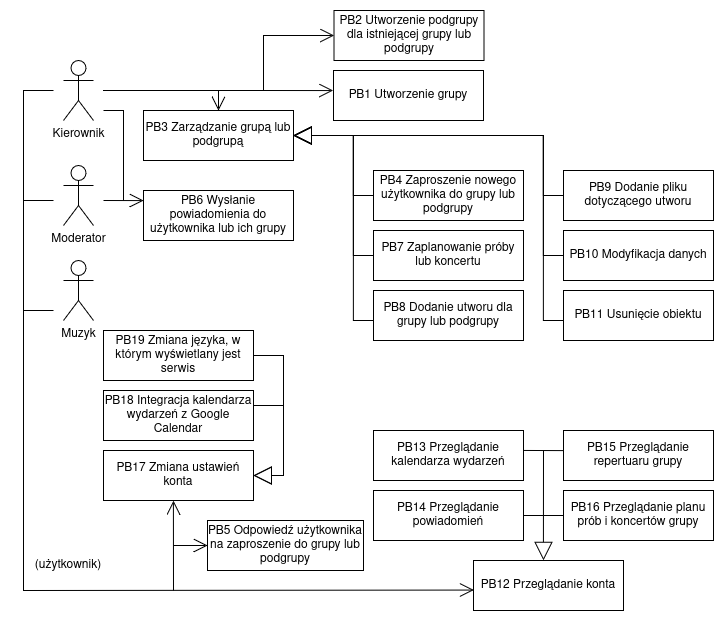
\includegraphics[width=0.95\linewidth]{images/diagram_przypadkow_biznesowych.png}
    \caption{Diagram przypadków biznesowych}
\end{figure}

\begin{figure} [H]
    \centering
    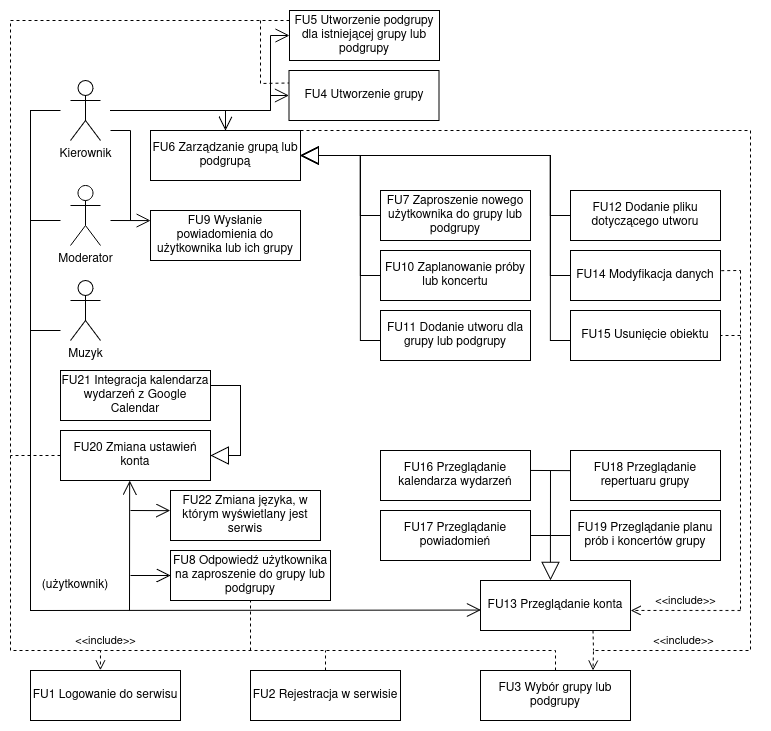
\includegraphics[width=0.95\linewidth]{images/diagram_przypadkow_systemowych.png}
    \caption{Diagram przypadków systemowych}
\end{figure}

\subsubsection{PB1. Utworzenie grupy}

Aktorzy: kierownik.
\begin{enumerate}
    \item System weryfikuje tożsamość kierownika.
    \item Kierownik podaje informacje o grupie, którą zamierza utworzyć.
    \item System tworzy grupę z kierownikiem jako jej przewodniczącym i jedynym członkiem.
\end{enumerate}

\subsubsection{PB2. Utworzenie podgrupy dla istniejącej grupy lub podgrupy}

Aktorzy: kierownik.
\begin{enumerate}
    \item System weryfikuje tożsamość kierownika.
    \item Kierownik wybiera (pod)grupę i podaje informacje o jej podgrupie, którą zamierza utworzyć.
    \item System tworzy podgrupę z kierownikiem jako jej przewodniczącym i jedynym członkiem.
\end{enumerate}

\subsubsection{PB3. Zarządzanie grupą lub podgrupą}

Przypadek generalizujący dla PB4, PB7-11.

Aktorzy: kierownik.
\begin{enumerate}
    \item System weryfikuje tożsamość kierownika.
    \item Kierownik wybiera grupę (lub podgrupę, jeżeli to nią chce zarządzać) oraz sekcję, w której chciałby dokonać zmian.
    \item Kierownik wykonuje akcję dotyczącą (pod)grupy.
\end{enumerate}

\subsubsection{PB4. Zaproszenie nowego użytkownika do grupy lub podgrupy}

Przypadek specjalizujący PB3.

Aktorzy: kierownik.
\begin{enumerate}
    \item Jak w przypadku generalizującym PB3 – kroki 1. i 2.
    \item Kierownik wybiera użytkownika, którego chciałby zaprosić do zespołu.
    \item System zapamiętuje zaproszenie, by móc je później przedstawić użytkownikowi.
\end{enumerate}

\subsubsection{PB5. Odpowiedź użytkownika na zaproszenie do grupy lub podgrupy}

Aktorzy: użytkownik.

Scenariusz główny:
\begin{enumerate}
    \item System weryfikuje tożsamość użytkownika.
    \item System powiadamia użytkownika o istniejącym zaproszeniu od kierownika do (pod)grupy.
    \item Użytkownik przyjmuje zaproszenie.
    \item System usuwa zaproszenie i dodaje użytkownika do (pod)grupy.
\end{enumerate}

Scenariusz alternatywny – użytkownik odrzuca zaproszenie:
\begin{enumerate}
    \item Jak w scenariuszu głównym – kroki 1. i 2.
    \item Użytkownik odrzuca zaproszenie.
    \item System usuwa zaproszenie bez dodawania użytkownika do (pod)grupy.
\end{enumerate}

\subsubsection{PB6. Wysłanie powiadomienia do użytkownika lub ich grupy}

Przypadek specjalizujący PB3.

Aktorzy: kierownik lub moderator (dalej zwany kierownikiem).
\begin{enumerate}
    \item Jak w przypadku generalizującym PB3 – kroki 1. i 2.
    \item Kierownik podaje adresatów, temat i treść powiadomienia oraz decyduje, czy wiadomość ma trafić również na skrzynkę e-mailową adresatów.
    \item System wysyła powiadomienie (również na skrzynkę pocztową, jeżeli tak zdecydował kierownik).
\end{enumerate}

\subsubsection{PB7. Zaplanowanie próby lub koncertu}

Przypadek specjalizujący PB3.

Aktorzy: kierownik.
\begin{enumerate}
    \item Jak w przypadku generalizującym PB3 – kroki 1. i 2.
    \item Kierownik podaje informacje o próbie/koncercie i uczestników wydarzenia (cała (pod)grupa lub lista członków).
    \item System zapamiętuje nowe dane.
\end{enumerate}

\subsubsection{PB8. Dodanie utworu dla grupy lub podgrupy}

Przypadek specjalizujący PB3.

Aktorzy: kierownik.
\begin{enumerate}
    \item Jak w przypadku generalizującym PB3 – kroki 1. i 2.
    \item Kierownik podaje informacje o utworze.
    \item System zapamiętuje nowe dane.
\end{enumerate}

\subsubsection{PB9. Dodanie pliku dotyczącego utworu}

Przypadek specjalizujący PB3.

Aktorzy: kierownik.
\begin{enumerate}
    \item Jak w przypadku generalizującym PB3 – kroki 1. i 2.
    \item Kierownik wybiera utwór i dodaje dotyczący go plik. Wybiera, kto ma mieć dostęp do pliku. Plik może zostać oznaczony nazwami instrumentów muzycznych oraz głosów.
    \item System zapamiętuje nowe dane.
\end{enumerate}

\subsubsection{PB10. Modyfikacja danych}

Przypadek specjalizujący PB3.

Aktorzy: kierownik.
\begin{enumerate}
    \item Jak w przypadku generalizującym PB3 – kroki 1. i 2.
    \item Kierownik nawiguje do wybranego obiektu - (pod)grupy, próby, koncertu, utworu, uprawnień użytkownika – i zmienia dla niego dane.
    \item System zapamiętuje wprowadzone zmiany.
\end{enumerate}

\subsubsection{PB11. Usunięcie obiektu}

Przypadek specjalizujący PB3.

Aktorzy: kierownik.
\begin{enumerate}
    \item Jak w przypadku generalizującym PB3 – kroki 1. i 2.
    \item Kierownik nawiguje do wybranego obiektu - (pod)grupy, próby, koncertu, utworu, uprawnień użytkownika – i wybiera jego usunięcie.
    \item System prosi o potwierdzenie wykonywanej akcji. Jeżeli zostanie anulowana – koniec scenariusza.
    \item System usuwa obiekt. Jeżeli usunięto (pod)grupę, usuwa się jej wszystkie powiadomienia, utwory, zaplanowane koncerty i próby. Jeżeli usunięto utwór, usuwa się wszystkie udostępnione do niego pliki.
\end{enumerate}

\subsubsection{PB12. Przeglądanie konta}

Przypadek generalizujący dla PB13-16.

Aktorzy: użytkownik.
\begin{enumerate}
    \item System weryfikuje tożsamość użytkownika.
    \item Jeżeli użytkownik jest zainteresowany informacjami dla konkretnej (pod)grupy, wybiera ją.
    \item Użytkownik przegląda interesujące go informacje.
\end{enumerate}

\subsubsection{PB13. Przeglądanie kalendarza wydarzeń}

Przypadek specjalizujący PB12.

Aktorzy: użytkownik.
\begin{enumerate}
    \item System weryfikuje tożsamość użytkownika.
    \item Użytkownik ogląda kalendarz z naniesionymi terminami zaplanowanych prób i koncertów w (pod)grupach, do których należy. Użytkownik może wybrać któreś wydarzenie, by uzyskać o nim więcej informacji.
\end{enumerate}

\subsubsection{PB14. Przeglądanie powiadomień}

Przypadek specjalizujący PB12.

Aktorzy: użytkownik.
\begin{enumerate}
    \item System weryfikuje tożsamość użytkownika.
    \item Użytkownik wybiera listę powiadomień dla wszystkich lub wybranej grupy i przegląda wiadomości. Może je również wyszukiwać.
\end{enumerate}


\subsubsection{PB15. Przeglądanie repertuaru grupy}

Przypadek specjalizujący PB12.

Aktorzy: użytkownik.
\begin{enumerate}
    \item System weryfikuje tożsamość użytkownika.
    \item Użytkownik wybiera (pod)grupę, której repertuar chce przeglądać.
    \item Użytkownik wyświetla wszystkie utwory lub zawęża poszukiwania za pomocą nazwy utworu, wykorzystywanego instrumentu lub koncertu, na którym ma być wykonywany.
    \item Użytkownik może wybrać utwór oraz przeglądać i pobierać podpięte pod niego pliki, do których ma dostęp. Lista plików może również być filtrowana.
\end{enumerate}

\subsubsection{PB16. Przeglądanie planu prób i koncertów grupy}

Przypadek specjalizujący PB12.

Aktorzy: użytkownik.
\begin{enumerate}
    \item System weryfikuje tożsamość użytkownika.
    \item Użytkownik wybiera (pod)grupę, której planem wydarzeń jest zainteresowany.
    \item Użytkownik przegląda listę wydarzeń. Może je wyszukiwać oraz wybierać wydarzenia, by uzyskać na ich temat więcej informacji.
\end{enumerate}

\subsubsection{PB17. Zmiana ustawień konta}

Przypadek generalizujący dla PB18 i PB19.

Aktorzy: użytkownik.
\begin{enumerate}
    \item System weryfikuje tożsamość użytkownika.
    \item Użytkownik modyfikuje ustawienia konta i zatwierdza zmiany.
    \item System wprowadza zmiany w życie.
\end{enumerate}

\subsubsection{PB18. Integracja kalendarza wydarzeń z Google Calendar}

Przypadek specjalizujący PB17.

Aktorzy: użytkownik.
\begin{enumerate}
    \item System weryfikuje tożsamość użytkownika.
    \item Użytkownik udostępnia systemowi swój Kalendarz Google.
    \item System wstawia wydarzenia użytkownika do kalendarza i umożliwia ich aktualizację.
\end{enumerate}

\subsubsection{PB19. Zmiana języka, w którym wyświetlany jest serwis}

Przypadek specjalizujący PB17.

Aktorzy: użytkownik.
\begin{enumerate}
    \item Użytkownik wybiera język, w którym chciałby korzystać z serwisu.
    \item System realizuje zmianę języka.
\end{enumerate}

\subsubsection{FU1. Logowanie do serwisu}

Wspiera procedury PB1-18.

Aktorzy: użytkownik.

Scenariusz główny:
\begin{enumerate}
    \item Użytkownik wybiera opcję logowania poprzez Google.
    \item System autoryzacji Google wyświetla okno logowania.
    \item Użytkownik podaje konto, którym chce się logować. Jeżeli nie jest jeszcze na nim zalogowany, podaje potrzebne do tego dane.
    \item System otrzymuje od Google informację o poprawnym zalogowaniu i umożliwia użytkownikowi korzystanie z serwisu.
\end{enumerate}

\subsubsection{FU2. Rejestracja w serwisie}

Wspiera procedury PB1-18. Korzysta z FU1.

Aktorzy: użytkownik.
\begin{enumerate}
    \item Użytkownik loguje się poprzez Google (FU1).
    \item System nie znajduje użytkownika w bazie danych, więc tworzy konto, wypełnia pola z danymi osobowymi informacjami uzyskanymi z konta Google oraz odsyła do głównej części serwisu.
\end{enumerate}

\subsubsection{FU3. Wybór grupy lub podgrupy}

Wspiera procedury PB2-4, PB6-12, PB15, PB16. Korzysta z FU1.

Aktorzy: użytkownik.
\begin{enumerate}
    \item Użytkownik loguje się do serwisu (FU1).
    \item System prezentuje okno z grupami i ich podgrupami, których członkiem jest użytkownik.
    \item Użytkownik wybiera (pod)grupę, którą jest zainteresowany oraz sekcję, w której zamierza wykonać akcję (struktura grupy, wydarzenia, utwory i pliki, dodanie wiadomości)
    \item System przenosi użytkownika do odpowiedniego panelu wybranej grupy.
\end{enumerate}

\subsubsection{FU4. Utworzenie grupy}

Wspiera procedury PB1 – Utworzenie grupy i PB2 – Utworzenie podgrupy dla istniejącej grupy. Korzysta z FU1.

Aktorzy: kierownik.
\begin{enumerate}
    \item Kierownik loguje się do serwisu (FU1).
    \item System prezentuje okno z grupami i ich podgrupami, których członkiem jest kierownik.
    \item Kierownik wybiera opcję utworzenia nowej grupy.
    \item System wyświetla formularz z informacjami o grupie.
    \item Kierownik podaje nazwę i opis grupy.
    \item System tworzy grupę z kierownikiem jako jej przewodniczącym i jedynym członkiem oraz odsyła do okna z (pod)grupami.
\end{enumerate}

\subsubsection{FU5. Utworzenie podgrupy dla istniejącej grupy lub podgrupy}

Wspiera procedurę PB2 – Utworzenie podgrupy dla istniejącej grupy. Korzysta z FU1.

Aktorzy: kierownik.
\begin{enumerate}
    \item Kierownik loguje się do serwisu (FU1).
    \item System prezentuje okno z grupami i ich podgrupami, których członkiem jest kierownik.
    \item Kierownik wybiera opcję zarządzania (pod)grupą i w niej opcję utworzenia podgrupy.
    \item System wyświetla formularz z informacjami o podgrupie.
    \item Kierownik podaje nazwę i opis podgrupy.
    \item System tworzy podgrupę z kierownikiem jako jej przewodniczącym i jedynym członkiem oraz odsyła do okna z (pod)grupami.
\end{enumerate}

\subsubsection{FU6. Zarządzanie grupą lub podgrupą}

Wspiera procedurę PB3 – Zarządzanie grupą lub podgrupą. Korzysta z FU1 i FU3. Funkcja generalizująca dla FU7 i FU10-14.

Aktorzy: kierownik.
\begin{enumerate}
    \item Kierownik loguje się do serwisu (FU1) i wybiera (pod)grupę (FU3).
    \item Kierownik nawiguje do odpowiedniego miejsca w sekcji i wykonuje interesującą go akcję.
    \item System realizuje zadaną akcję.
\end{enumerate}

\subsubsection{FU7. Zaproszenie nowego użytkownika do grupy lub podgrupy}

Wspiera procedurę PB4 – Zaproszenie nowego muzyka do grupy lub podgrupy. Funkcja specjalizująca FU6.

Aktorzy: kierownik.
\begin{enumerate}
    \item Jak w funkcji generalizującej FU6 – krok 1.
    \item Kierownik wybiera opcję zaproszenia nowego użytkownika w sekcji zarządzania (pod)grupą.
    \item System wyświetla formularz do utworzenia zaproszenia.
    \item Kierownik podaje adres e-mail adresata zaproszenia, zaznacza poziom uprawnień, jaki powinien otrzymać i zatwierdza akcję.
    \item System generuje zaproszenie i odsyła do sekcji z informacjami o (pod)grupie.
\end{enumerate}

\subsubsection{FU8. Odpowiedź użytkownika na zaproszenie do grupy lub podgrupy}

Wspiera procedurę PB5 – Odpowiedź użytkownika na zaproszenie do grupy lub podgrupy. Korzysta z FU1.

Aktorzy: użytkownik.

Scenariusz główny:
\begin{enumerate}
    \item Użytkownik loguje się do serwisu (FU1).
    \item System wyświetla okno z grupami, gdzie znajduje się informacja o zaproszeniu.
    \item Użytkownik przyjmuje zaproszenie.
    \item System usuwa zaproszenie i dodaje użytkownika do (pod)grupy.
\end{enumerate}

Scenariusz alternatywny – muzyk odrzuca zaproszenie:
\begin{enumerate}
    \item Jak w scenariuszu głównym – kroki 1. i 2.
    \item Użytkownik odrzuca zaproszenie.
    \item System usuwa zaproszenie bez dodawania użytkownika do (pod)grupy.
\end{enumerate}

\subsubsection{FU9. Wysłanie powiadomienia do użytkownika lub ich grupy}

Wspiera procedurę PB6 – Wysłanie powiadomienia do użytkownika lub ich grupy. Funkcja specjalizująca FU6.

Aktorzy: kierownik lub moderator (dalej zwany kierownikiem).
\begin{enumerate}
    \item Jak w funkcji generalizującej FU6 – krok 1.
    \item System udostępnia okno do napisania wiadomości.
    \item Kierownik wpisuje tytuł i treść wiadomości oraz wybiera, do kogo ją wysłać i czy również e-mailem.
    \item System zapisuje powiadomienie do przekazania adresatom (i wysyła im e-mail, jeżeli tak zdecydował kierownik) i zamyka okno.
\end{enumerate}

\subsubsection{FU10. Zaplanowanie próby lub koncertu}

Wspiera procedurę PB7 – Zaplanowanie próby lub koncertu. Funkcja specjalizująca FU6.

Aktorzy: kierownik.
\begin{enumerate}
    \item Jak w funkcji generalizującej FU6 – krok 1.
    \item Kierownik wybiera opcję utworzenia nowego wydarzenia w sekcji z wydarzeniami.
    \item System wyświetla formularz do utworzenia wydarzenia.
    \item Kierownik wpisuje tytuł wydarzenia, opis, czas, miejsce i uczestników (cała (pod)grupa lub jej wybrani członkowie).
    \item System dodaje próbę/koncert i odsyła do sekcji z wydarzeniami.
    \item Kierownik może zedytować wydarzenie i podpiąć pod nie wybrane utwory grupy - wtedy system zapisze dodatkowe informacje.
\end{enumerate}

\subsubsection{FU11. Dodanie utworu dla grupy lub podgrupy}

Wspiera procedurę PB8 – Dodanie utworu dla grupy lub podgrupy. Funkcja specjalizująca FU6.

Aktorzy: kierownik.
\begin{enumerate}
    \item Jak w funkcji generalizującej FU6 – krok 1.
    \item Kierownik wybiera opcję dodania nowego utworu w sekcji z utworami.
    \item System wyświetla formularz do dodania utworu.
    \item Kierownik wpisuje tytuł i twórcę utworu.
    \item System dodaje utwór i odsyła do zakładki z utworami.
\end{enumerate}

\subsubsection{FU12. Dodanie pliku dotyczącego utworu}

Wspiera procedurę PB9 – Dodanie pliku dotyczącego utworu. Funkcja specjalizująca FU6.

Aktorzy: kierownik.
\begin{enumerate}
    \item Jak w funkcji generalizującej FU6 – krok 1.
    \item W sekcji z utworami kierownik wybiera utwór, do którego chciałby dodać plik.
    \item System wyświetla informacje o utworze i listę plików.
    \item Kierownik wybiera opcję dodania nowego pliku.
    \item System wyświetla formularz do dodania nowego pliku.
    \item Kierownik wgrywa plik, może też podać instrumenty, którego dotyczy. Wybiera, którzy członkowie (pod)grupy mają mieć dostęp do pliku.
    \item System dodaje plik i odsyła do informacji o utworze.
\end{enumerate}

\subsubsection{FU13. Modyfikacja danych}

Wspiera procedurę PB10 – Modyfikacja danych. Funkcja specjalizująca FU6.

Aktorzy: kierownik.
\begin{enumerate}
    \item Jak w funkcji generalizującej FU6 – krok 1.
    \item Kierownik nawiguje do wybranego obiektu: próby, koncertu, utworu, pliku, informacji o (pod)grupie, uprawnień członka zespołu. Wybiera opcję edycji danych o zasobie.
    \item System wyświetla formularz ze starymi danymi o obiekcie.
    \item Kierownik podaje nowe dane na miejsce starych.
    \item System aktualizuje informacje o obiekcie i odsyła do miejsca, z którego wybrano opcję edycji.
\end{enumerate}

\subsubsection{FU14. Usunięcie obiektu}

Wspiera procedurę PB11 – Usunięcie obiektu. Funkcja specjalizująca FU6.

Aktorzy: kierownik.
\begin{enumerate}
    \item Jak w funkcji generalizującej FU6 – krok 1.
    \item Kierownik nawiguje do wybranego obiektu: próby, koncertu, utworu, pliku, członkostwa użytkownika, informacji o (pod)grupie (w przypadku usuwania całej (pod)grupy). Wybiera opcję usunięcia obiektu.
    \item System usuwa obiekt (w niektórych przypadkach prosi o potwierdzenie akcji - wtedy kierownik musi to zrobić). Jeżeli usunięto (pod)grupę, usuwa się jej wszystkie powiadomienia, utwory, zaplanowane koncerty i próby. Jeżeli usunięto utwór, usuwa się wszystkie udostępnione do niego pliki.
\end{enumerate}

\subsubsection{FU15. Przeglądanie konta}

Wspiera procedurę PB12 – Przeglądanie konta. Funkcja generalizująca FU16-20. Korzysta z FU1 i FU3.

Aktorzy: użytkownik.
\begin{enumerate}
    \item Użytkownik loguje się do serwisu (FU1) i wybiera (pod)grupę (FU3) lub inny panel.
    \item System wyświetla zadaną sekcję serwisu.
    \item Użytkownik przegląda interesujące go informacje.
\end{enumerate}


\subsubsection{FU16. Przeglądanie kalendarza wydarzeń}

Wspiera procedurę PB13 – Przeglądanie kalendarza wydarzeń. Funkcja specjalizująca FU15.

Aktorzy: użytkownik.
\begin{enumerate}
    \item Użytkownik loguje się do serwisu (FU1) i wybiera panel z kalendarzem wydarzeń.
    \item System wyświetla kalendarz z naniesionymi terminami zaplanowanych prób i koncertów w (pod)grupach, do których należy.
    \item Użytkownik przegląda informacje. Jeżeli wybierze datę, system wyświetli skrócone informacje o odbywających się wtedy wydarzeniach z możliwością przejścia do szczegółów o wydarzeniu.
\end{enumerate}

\subsubsection{FU17. Przeglądanie powiadomień}

Wspiera procedurę PB14 – Przeglądanie powiadomień. Funkcja specjalizująca FU15.

Aktorzy: użytkownik.
\begin{enumerate}
    \item Użytkownik loguje się do serwisu (FU1) i wybiera panel z listą powiadomień.
    \item System wyświetla wysłane użytkownikowi powiadomienia z tytułem, informacją o autorze, (pod)grupie pochodzenia i datą wysłania.
    \item Użytkownik przegląda informacje. Może przeprowadzić wyszukiwanie wiadomości po tytule, nadawcy i (pod)grupie pochodzenia, podając odpowiednie frazy.
    \item Jeżeli przeprowadzono wyszukiwanie, system wyświetla przefiltrowane dane.
\end{enumerate}

\subsubsection{FU18. Przeglądanie repertuaru grupy}

Wspiera procedurę PB15 – Przeglądanie repertuaru grupy. Funkcja specjalizująca FU15.

Aktorzy: użytkownik.
\begin{enumerate}
    \item Użytkownik loguje się do serwisu (FU1) i wybiera (pod)grupę (FU3).
    \item System wyświetla sekcję z utworami.
    \item Użytkownik przegląda utwory. Może przeprowadzić wyszukiwanie (po nazwie utworu, wykorzystywanego instrumentu lub powiązanego koncertu) lub wybrać utwór.
    \item Jeżeli przeprowadzono wyszukiwanie, system wyświetla przefiltrowane dane. Jeżeli wybrano utwór, system wyświetla informacje o nim i listę podpiętych pod niego plików, do których użytkownik ma zdefiniowany dostęp.
\end{enumerate}

\subsubsection{FU19. Przeglądanie planu prób i koncertów grupy}

Wspiera procedurę PB16 – Przeglądanie planu prób i koncertów grupy. Funkcja specjalizująca FU15.

Aktorzy: użytkownik.
\begin{enumerate}
    \item Użytkownik loguje się do serwisu (FU1) i wybiera (pod)grupę (FU3).
    \item System wyświetla sekcję z wydarzeniami.
    \item Użytkownik przegląda listę wydarzeń z naniesionymi informacjami o nich. Może wybierać wydarzenia albo przeprowadzić wyszukiwanie (po nazwie, miejscu i opisie).
    \item Jeżeli wybrano wydarzenie, system wyświetla listę powiązanych plików, do których użytkownik ma dostęp. Jeżeli przeprowadzono wyszukiwanie, system wyświetla przefiltrowane dane. 
\end{enumerate}

\subsubsection{FU20. Zmiana ustawień konta}

Wspiera procedurę PB17 – Zmiana ustawień konta. Korzysta z FU1. Przypadek generalizujący dla FU21.

Aktorzy: użytkownik.
\begin{enumerate}
    \item Użytkownik loguje się do serwisu (FU1) i wybiera panel z ustawieniami.
    \item System wyświetla możliwe pola do edycji.
    \item Użytkownik podaje nowe dane i zatwierdza zmiany.
    \item System zapisuje nowe informacje.
\end{enumerate}

\subsubsection{FU21. Integracja kalendarza wydarzeń z Google Calendar}

Wspiera procedurę PB18 – Integracja kalendarza wydarzeń z Google Calendar. Specjalizuje FU20.

Aktorzy: użytkownik.
\begin{enumerate}
    \item Jak w funkcji generalizującej FU20 – kroki 1. i 2.
    \item Użytkownik wybiera konto Google, by podłączyć jego kalendarz.
    \item System wstawi do kalendarza listę wydarzeń dotyczących użytkownika. Można wybrać opcję synchronizacji, by ją zaktualizować.
\end{enumerate}

\subsubsection{FU22. Zmiana języka, w którym wyświetlany jest serwis}

Wspiera procedurę PB19 – Zmiana języka, w którym wyświetlany jest serwis.

Aktorzy: użytkownik.
\begin{enumerate}
    \item Użytkownik wybiera listę języków.
    \item System wyświetla wszystkie dostępne języki, w których można korzystać z serwisu.
    \item Użytkownik zaznacza jeden z języków.
    \item System zmienia język serwisu.
\end{enumerate}

\subsection{Potwierdzenie zgodności wymagań}

\begin{figure} [H]
    \centering
    
\includegraphics[width=0.95\linewidth]{images/potwierdzenie.png}
    \caption{Wiadomości potwierdzające wymagania}
\end{figure}

\section{Definicja architektury}

Rozwiązanie jest oparte o architekturę trójwarstwową – użytkownik łączy się poprzez sieć z serwerem NGINX udostępniającym pliki statyczne aplikacji webowej w React.js. Gdy użytkownik wykona akcję wymagająca wysłania zapytania, ten sam serwer przekazuje przychodzące zapytanie poprzez reverse proxy i load balancer do REST API obsługiwanego przez Django. Komponenty backendowe mogą wykonywać operacje CRUD na bazie danych w PostgreSQL (która może być rozdzielona na serwery master i slave).

Jednymi z wymagań dotyczących systemu są skalowalność i wydajność przy setkach użytkowników. Konieczna jest więc architektura wspierająca zwiększanie mocy obliczeniowej wraz z rosnącym ruchem w aplikacji – obsługa zapytań odbywa się na wielu maszynach wirtualnych, a ruch jest rozdzielany za pomocą load balancerów. Zdecydowaliśmy się na skorzystanie z usług chmurowych Azure do utworzenia maszyn wirtualnych, na których będą wdrażane poszczególne komponenty:

\begin{figure} [H]
    \centering
    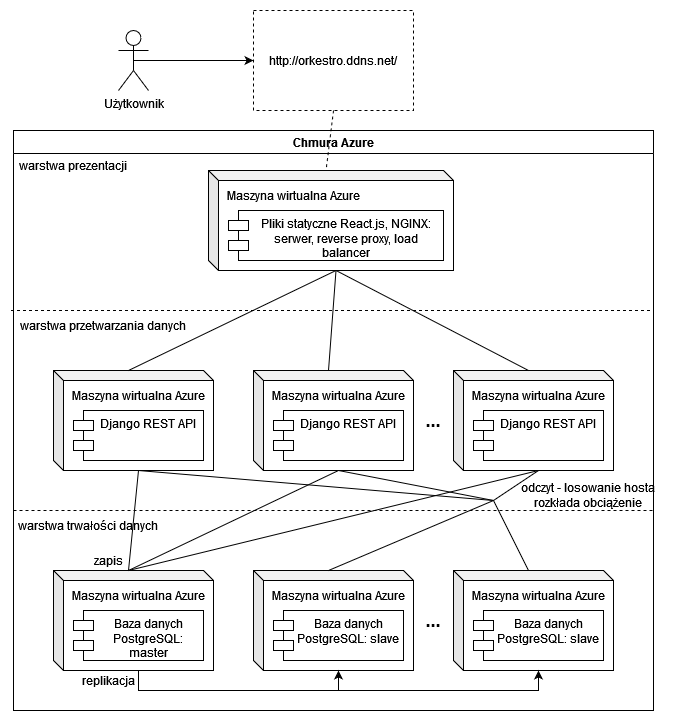
\includegraphics[width=0.95\linewidth]{images/arch.png}
    \caption{Diagram architektury systemu w postaci ogólnej}
\end{figure}

Każda maszyna z REST API może obsługiwać wszystkie zapytania - celem korzystania z wielu maszyn jest możliwość przetworzenia większej liczby zapytań naraz. Moduły REST API dostępne dla użytkownika:

\begin{figure} [H]
    \centering
    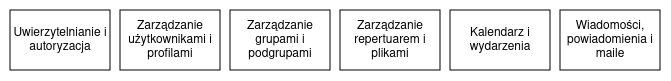
\includegraphics[width=0.95\linewidth]{images/rest.png}
    \caption{Podział zapytań do REST API na moduły}
\end{figure}

Wszystkie maszyny wirtualne pracują na Ubuntu Server 24.04. Użytkownik do połączenia z serwisem używa dowolnego urządzenia obsługującego rozsądnie aktualną i znaną przeglądarkę internetową. Możliwe jest dodawanie i usuwanie maszyn odpowiedzialnych za REST API.

Koszt pracy jednej, najtańszej dostępnej maszyny to około 210 zł miesięcznie, ale korzystając z Azure Spot można go obniżyć do około 29 zł miesięcznie w zamian za niedostępność maszyny przez około 5\% czasu. Korzystanie z publicznego adresu IP jest na ten moment darmowe, ale od października 2025 r. będzie kosztować około 14 zł miesięcznie. Do testowych wdrożeń korzystamy z kont studenckich, na których mamy dostęp do darmowych środków. Życzeniem klienta była możliwość minimalizacji kosztów utrzymania serwisu uruchomionego dla niewielkiej liczby użytkowników. Sposób połączenia komponentów umożliwia więc w szczególności uruchomienie wszystkich potrzebnych procesów na jednej maszynie wirtualnej:

\begin{figure} [H]
    \centering
    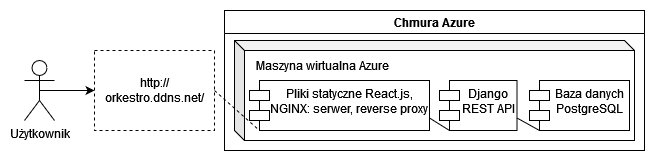
\includegraphics[width=0.95\linewidth]{images/arch_min.png}
    \caption{Diagram architektury systemu w uproszczonej postaci}
\end{figure}

\section{Dane trwałe}

\subsection{Model logiczny danych}

\begin{figure} [H]
    \centering
    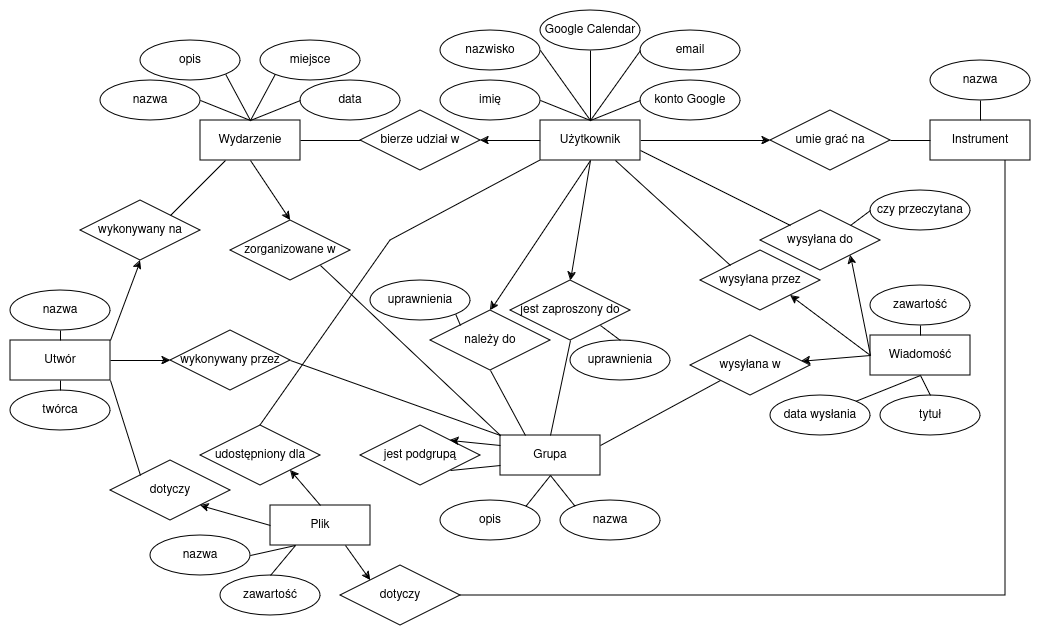
\includegraphics[width=0.95\linewidth]{images/er.png}
    \caption{Model koncepcyjny danych}
\end{figure}

\begin{figure} [H]
    \centering
    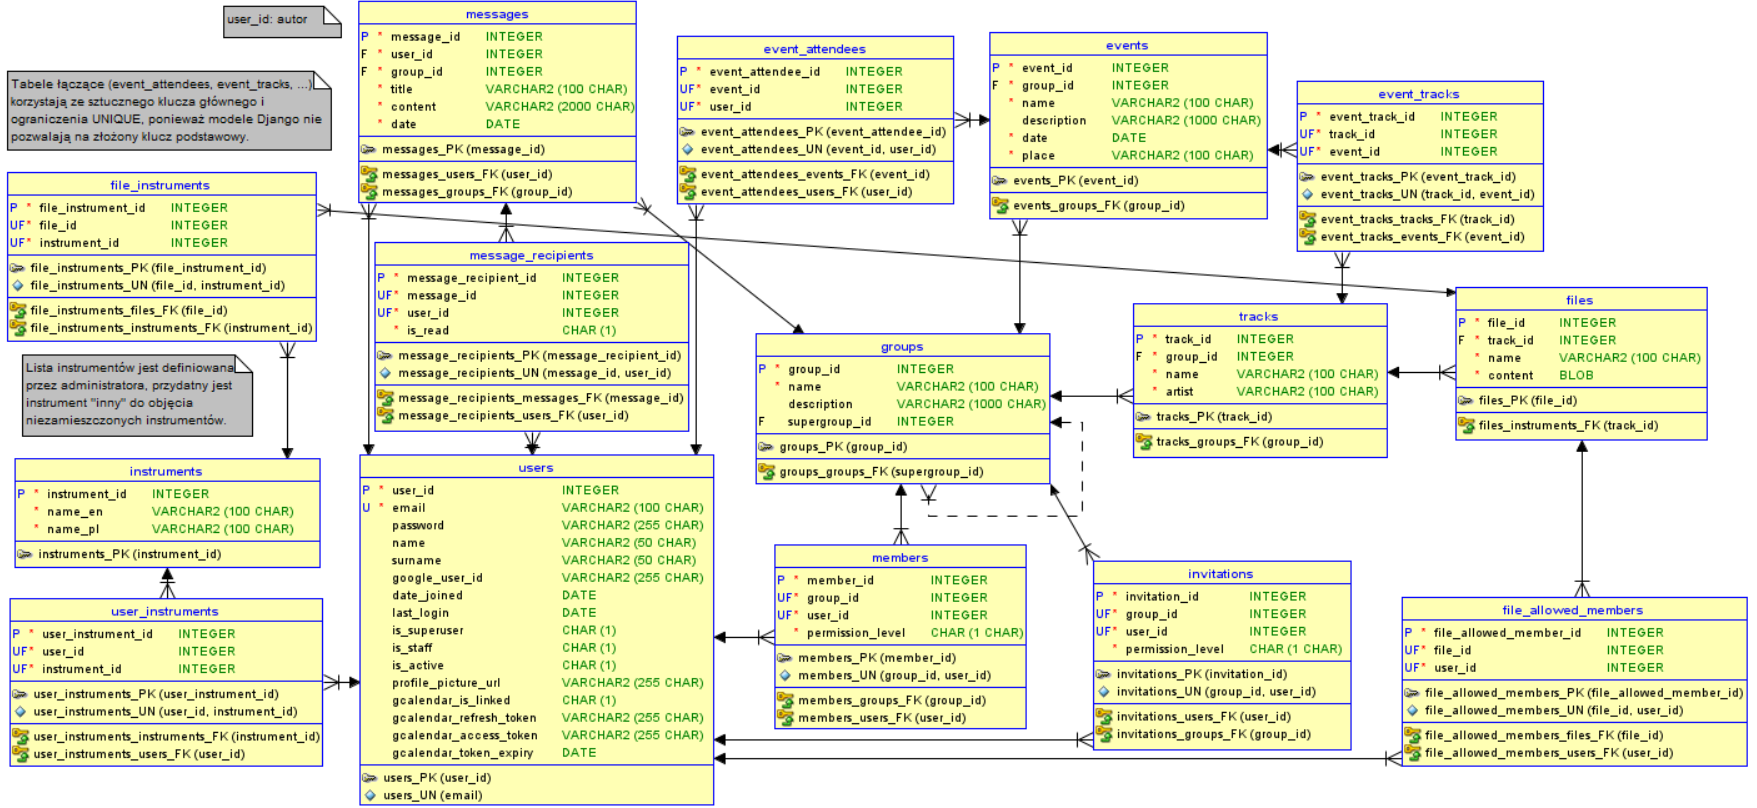
\includegraphics[width=0.95\linewidth]{images/logical.png}
    \caption{Model logiczny danych}
\end{figure}

Rekordy w tabelach łączących (\texttt{user\_instruments}, \texttt{file\_allowed\_members}, \texttt{file\_instruments}, \texttt{members}, \texttt{message\_recipients}, \texttt{invitations}, \texttt{event\_attendees}, \texttt{event\_tracks}) są kaskadowo usuwane przy usunięciu rekordu, do którego odwołuje się którykolwiek klucz obcy. Usunięcie utworu powoduje usunięcie podpiętych pod niego plików. Usunięcie grupy powoduje usunięcie podpiętych pod nią wiadomości, wydarzeń i utworów.

Wymaganiem projektu jest wydajność i skalowalność serwisu. Ponieważ ma być zaprojektowany jak dla setek jednoczesnych użytkowników, przydatne będzie zaindeksowanie tabel tak, by ułatwić wyszukiwanie danych. Wszystkie indeksy są typu mieszającego – większość danych jest w drzewiasty sposób podpięta do pewnej grupy lub użytkownika i wyszukiwanie będzie miało postać znalezienia rekordów z konkretną wartością klucza obcego. Nałożone indeksy:
\begin{itemize}
    \item w tabelach \texttt{user\_instruments}, \texttt{members}, \texttt{invitations}, \texttt{message\_recipients}, \texttt{event\_attendees}, \texttt{file\_allowed\_members} – na kolumnie \texttt{user\_id} (do znajdowania danych z perspektywy użytkownika)
    \item w tabelach \texttt{members}, \texttt{invitations}, \texttt{events}, \texttt{tracks} – na kolumnie \texttt{group\_id} (do znajdowania danych z perspektywy grupy)
    \item w tabelach \texttt{event\_tracks}, \texttt{event\_attendees} – na kolumnie \texttt{event\_id} (do znajdowania utworów i użytkowników związanych z wydarzeniem)
    \item w tabeli \texttt{event\_tracks} – na kolumnie \texttt{track\_id} (do znajdowania wydarzeń dla danego utworu)
    \item w tabeli \texttt{file\_allowed\_members}, \texttt{file\_instruments} – na kolumnie \texttt{file\_id} (do znajdowania instrumentów i użytkowników, którym udostępniono plik)
\end{itemize}

Oprócz wymienionych indeksów baza danych sama tworzy kolejne na kluczach głównych i kolumnach z unikalnymi wartościami (np. \texttt{email} w \texttt{users}, co przyspiesza wyszukiwanie użytkownika po autoryzacji Google).

\subsection{Przetwarzanie i przechowywanie danych}

Wybraliśmy relacyjną bazę danych PostgreSQL, z którą warstwa przetwarzania danych w Django będzie się łączyć poprzez adapter \texttt{psycopg}. Nie przewidujemy programowania w bazie danych (optymalizacja zapytań, triggery, procedury składowane).

\section{Specyfikacja analityczna i projektowa}

Repozytorium projektu: \href{https://gitlab-stud.elka.pw.edu.pl/zgromadzeni/orkestro}{https://gitlab-stud.elka.pw.edu.pl/zgromadzeni/orkestro}

Dokumentacja odnosi się do stanu projektu z commita 6ff754d0ebdb7423ccd548339ed071aa2305f2cf

\subsection{Metody realizacji}

Wykorzystywane metody realizacji:
\begin{itemize}
    \item serwer, load balancer, reverse proxy: NGINX
    \item technologie frontendowe: aplikacja webowa - React.js, Typescript, Tailwind CSS
    \item technologie backendowe: REST API - Python, Django, Django REST Framework
    \item testowanie: unittest, coverage.py
    \item baza danych: PostgreSQL
    \item dokumentacja: LaTeX, draw.io, SQL Developer Data Modeler
    \item praca grupowa, komunikacja: Git, GitLab, Messenger, Overleaf
    \item środowiska programowania: PyCharm, gedit, Neovim
    \item systemy operacyjne: Windows (10, 11), Linux (Ubuntu, Arch Linux, Fedora)
    \item uruchomienie, wdrożenie (lokalnie i na chmurę Azure): Docker, Docker Compose, skrypty bashowe
\end{itemize}

\subsection{Struktura klas}

W backendzie występuje duża liczba klas, które można podzielić na grupy funkcjonalne - dla lepszej przejrzystości struktura klas zostanie przedstawiona na kilku diagramach dla każdej takiej grupy. Na diagramach pojawią się klasy dostarczone przez Django, ponieważ praca z tym frameworkiem opiera się o pisanie klas pochodnych dostosowujących typowo spotykaną funkcjonalność aplikacji do danego projektu i oferujących dodatkowe funkcje. Wiele z tych klas ma dużą liczbę pól i metod oraz złożony schemat dziedziczenia - dla uproszczenia pokazujemy bezpośrednią nadklasę z własnymi/odziedziczonymi elementami istotnymi dla aplikacji.

Jako argumenty czy zwracane typy funkcji wykorzystywane są dodatkowe klasy Django, których struktura nie pojawi się na diagramach:
\begin{itemize}
\item request/Request: zapytanie HTTP
\item Response: odpowiedź HTTP
\item view/View - wywoływalna klasa przetwarzająca zapytanie
\item QuerySet - dane z zapytania do bazy danych
\item BaseAuthentication - klasa przeprowadzająca autoryzację użytkownika
\item Error - wiadomość o błędzie przy operacji na obiekcie typu Model
\item CharField, AutoField, ForeignKey, BooleanField, DateTimeField, BinaryField, EmailField, URLField - klasy obsługujące poszczególne typy danych w bazie
\item ReadOnlyPasswordHashField - klasa przechowująca hasło w formularzach panelu administratora.
\item BaseManager - klasa pobierająca listy rekordów z bazy danych
\end{itemize}

"Zbiorczy" diagram klas (poszczególne grupy klas zebrane pod jedną nazwą, zaznaczone związki występują w pewnej formie pomiędzy klasami w grupach):

\begin{figure} [H]
    \centering
    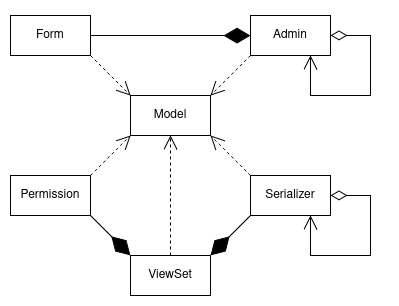
\includegraphics[width=0.4\linewidth]{images/general.png}
    \caption{Ogólny diagram klas}
\end{figure}

\subsubsection{Model}

Klasy dziedziczące po \texttt{Model} pośredniczą w wymianie danych z bazą. Na tak zdefiniowanych klasach Django ORM umożliwia m.in. pobieranie wszystkich lub jednego rekordu, modyfikację danych, dostęp do danych w powiązanych tabelach czy filtrowanie wszystkich rekordów po różnych kryteriach. Każdy model jest powiązany z tabelą w bazie, zdefiniowane są właściwości pól i więzy integralności. Zdefiniowane modele mają wyłączoną możliwość zarządzania cyklem życia tabel.

Klasa User wymagała dodatkowych pól i metod, by realizować operacje związane z autoryzacją użytkowników (m.in. hash hasła wymagany przez Django, ale niewykorzystywany przez nas, ponieważ korzystamy z logowania przez Google).

\begin{figure} [H]
    \centering
    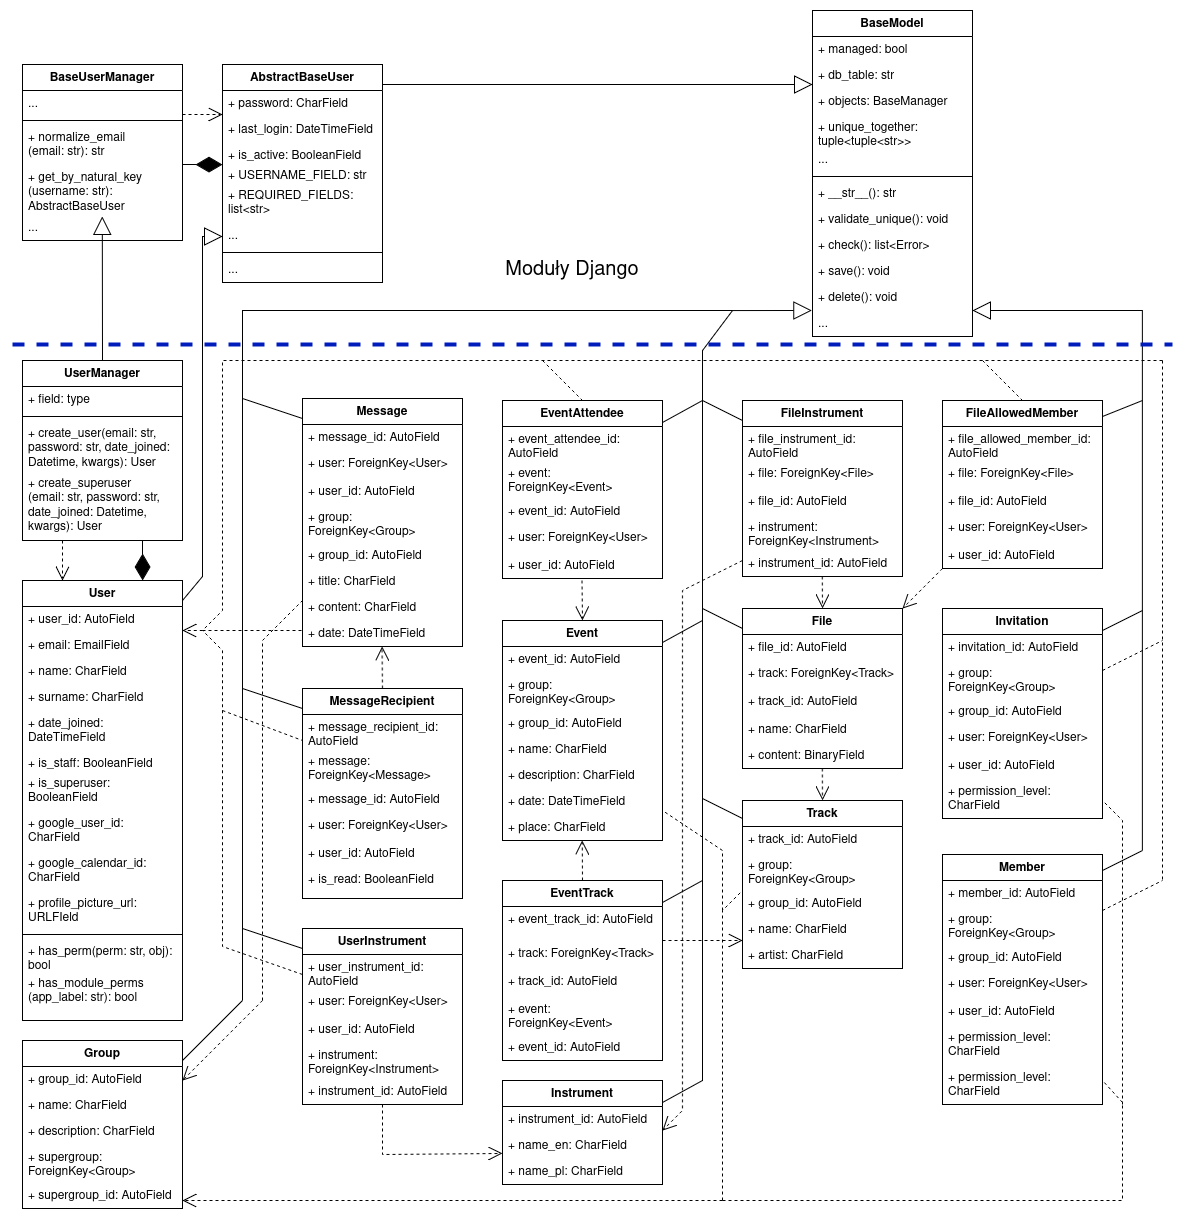
\includegraphics[width=0.95\linewidth]{images/models.png}
    \caption{Struktura klas typu Model}
\end{figure}

\subsubsection{Serializer}

Klasy dziedziczące po \texttt{ModelSerializer} służą do ładowania i zapisywania danych modeli do formatu JSON. Każdy serializator ma przypisany model, listę jego uwzględnianych pól i listę pól tylko do odczytu. Część klas przekazuje przy odczycie również dane z powiązanych tabel w bazie (poprzez dodatkowe pole), aby uniknąć dodatkowych zapytań do API. Jeżeli powiązany \texttt{ViewSet} umożliwia tworzenie i modyfikację danych modelu, tworzy się dwa serializatory - z wyszczególnionymi polami tylko do odczytu i bez nich.

\begin{figure} [H]
    \centering
    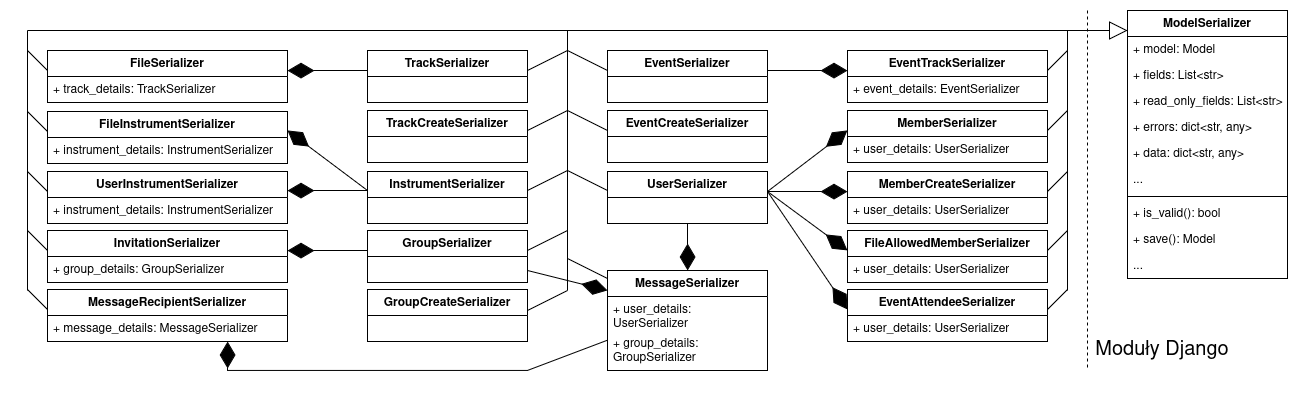
\includegraphics[width=0.95\linewidth]{images/serializers.png}
    \caption{Struktura klas typu Serializer}
\end{figure}

\subsubsection{Permission}

Klasy dziedziczące po \texttt{BasePermission} służą do weryfikacji, czy użytkownik ma uprawnienia do wykonania danej akcji w \texttt{ViewSet} (wszystkie zawarte w nim klasy muszą na to pozwolić, by zrealizować zapytanie). Uprawnienie może dotyczyć zapytań zbiorowych i konkretnego obiektu.

\begin{figure} [H]
    \centering
    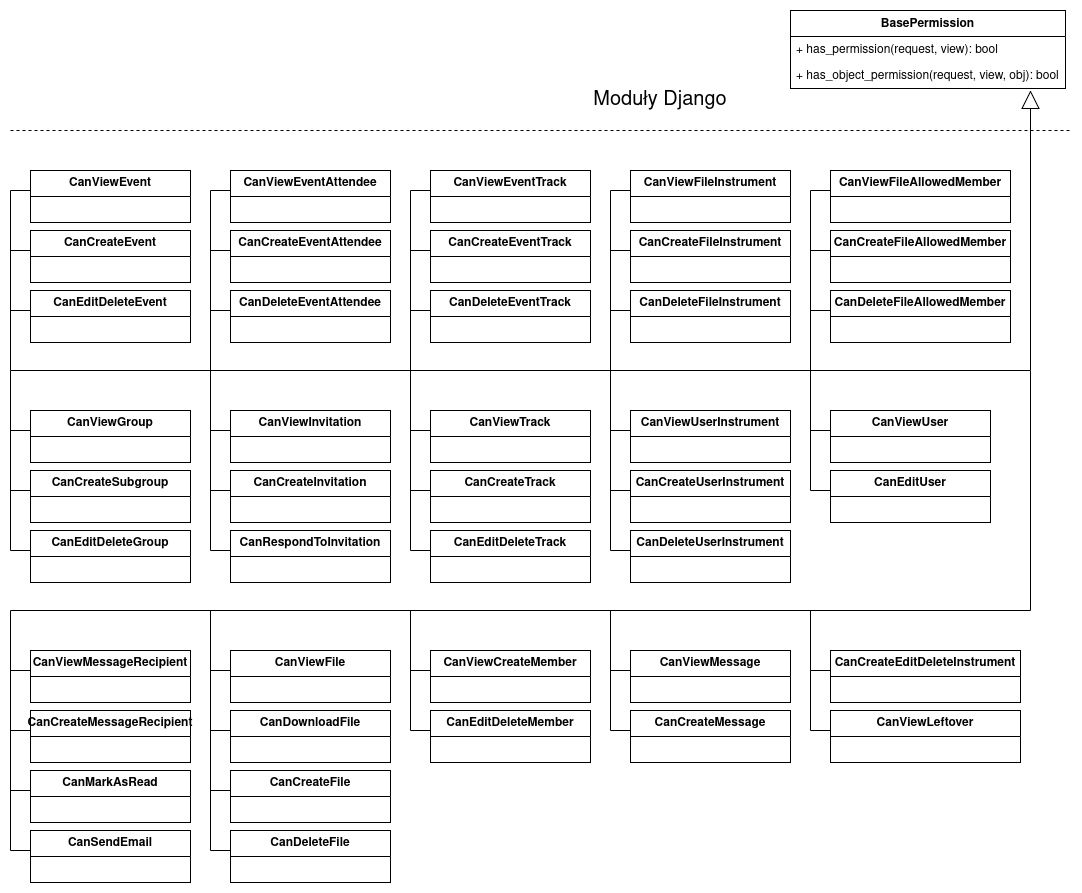
\includegraphics[width=0.95\linewidth]{images/permissions.png}
    \caption{Struktura klas typu Permission}
\end{figure}

\subsubsection{ViewSet}

Klasy dziedziczące po \texttt{ModelViewSet} zajmują się realizacją zapytań wysyłanych do endpointów - weryfikują uprawnienia użytkownika, przetwarzają dane i wysyłają odpowiedź. Każda niestatyczna metoda z argumentem \texttt{request} odpowiada za pewien endpoint, przy czym niektóre operacje są zablokowane poprzez niewpisanie odpowiedniej metody HTTP do \texttt{http\_method\_names}.

\begin{figure} [H]
    \centering
    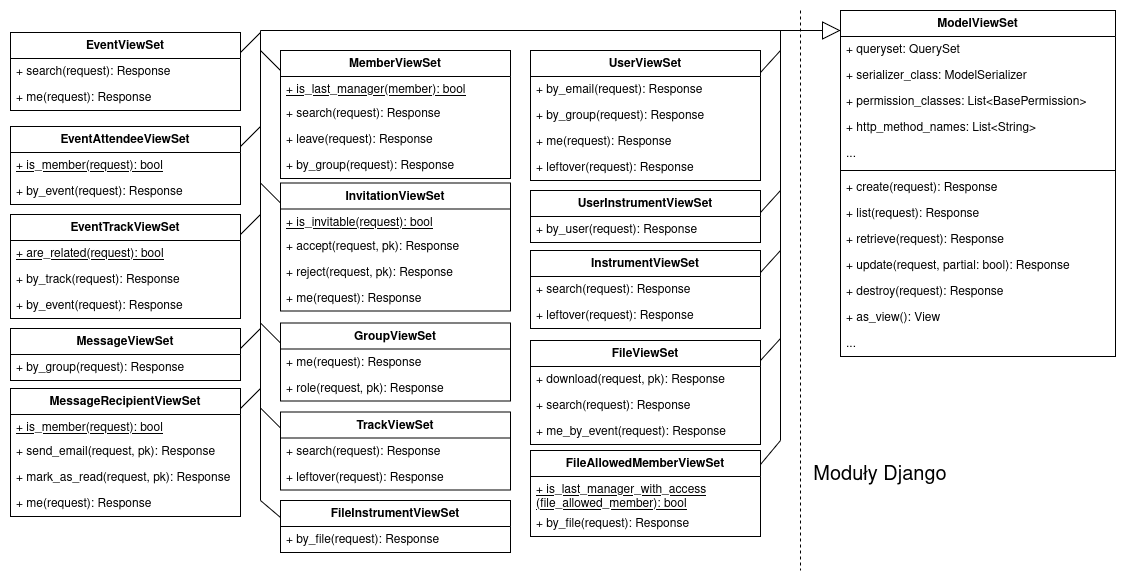
\includegraphics[width=0.95\linewidth]{images/viewsets.png}
    \caption{Struktura klas typu ViewSet}
\end{figure}

\subsubsection{Form, Admin}
Zdefiniowane klasy modyfikują domyślną funkcjonalność panelu administratora Django - umożliwiają dodanie podrzędnych obiektów podczas przeglądania nadrzędnego, modyfikują zakładkę z danymi użytkownika.

\begin{figure} [H]
    \centering
    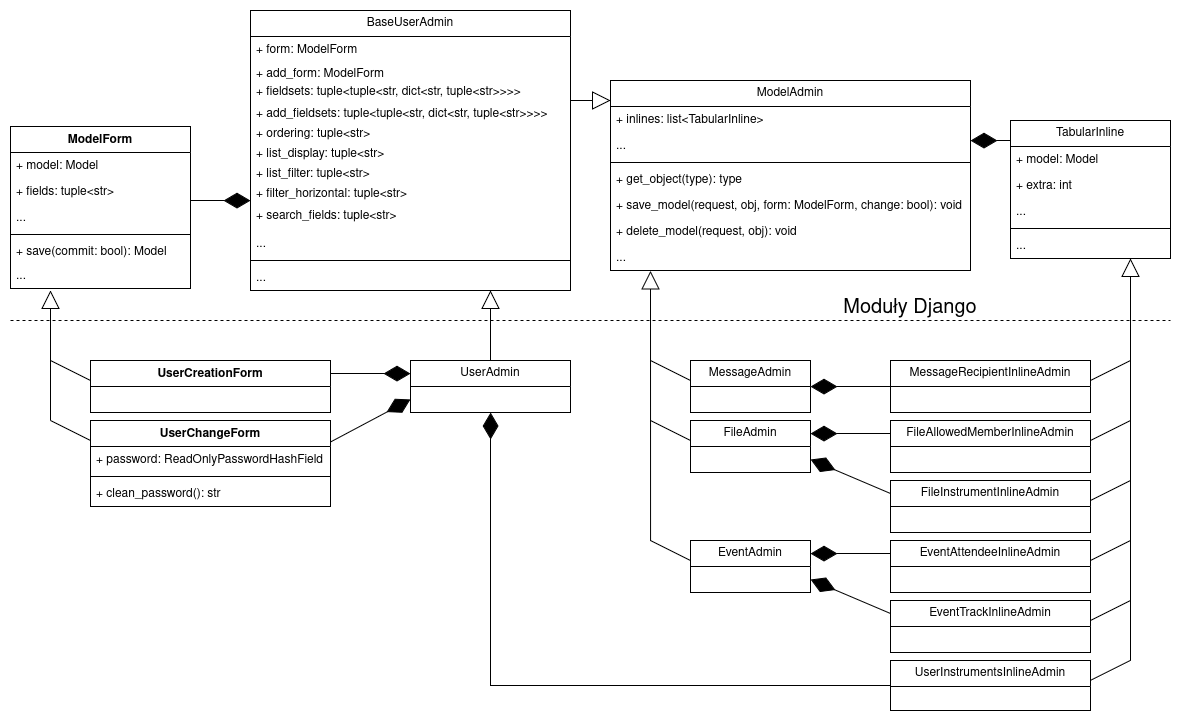
\includegraphics[width=0.95\linewidth]{images/forms_admin.png}
    \caption{Struktura klas typu Form/Admin}
\end{figure}

\subsubsection{Pozostałe}

Klasy nieujęte w pozostałych grupach:
\begin{itemize}
    \item \texttt{ApiConfig} - dziedziczy po \texttt{AppConfig}, ustawia niektóre pola w domyślnej konfiguracji aplikacji.
    \item \texttt{JWTCookieMiddleware} - dziedziczy po \texttt{MiddlewareMixin}, autoryzuje użytkownika przy dostępie do panelu administratora.
    \item \texttt{JWTCookieAuth} - dziedziczy po \texttt{JWTAuthentication}, autoryzuje użytkownika przy dostępie do API.
    \item \texttt{GoogleLoginView} - dziedziczy po \texttt{APIView}, (\texttt{View} - uproszczona wersja \texttt{ViewSet}, gdzie większa część kodu jest do samodzielnego napisania); umożliwia logowanie się kontem Google
    \item \texttt{GoogleLoginView} - dziedziczy po \texttt{APIView}, umożliwia podłączenie kalendarza Google
    \item \texttt{ReplicationRouter} - odpowiada za decydowanie, czy dane zapytanie wysłać do bazy danych master czy slave.
\end{itemize}

\subsection{Statystyki}

Statystyki dotyczące plików projektu:
\begin{itemize}
    \item liczba plików: 207
    \item linie kodu: 58104 (bez pliku \texttt{package\_lock.json}: 40010, bez pliku \texttt{package\_lock.json} i folderu z dokumentacją: 17946)
    \item liczba testów jednostkowych: 151
\end{itemize}

\section{Projekt standardu interfejsu użytkownika}

\subsection{Projekt UX}

User stories:
\begin{itemize}
	\item Jako kierownik chcę tworzyć (pod)grupy użytkowników, aby nimi zarządzać.
	\item Jako kierownik chcę planować wydarzenia dotyczące (pod)grupy, aby informować użytkowników o nadchodzących próbach czy koncertach.
	\item Jako kierownik chcę definiować utwory wykonywane przez (pod)grupę, aby informować użytkowników o obecnym repertuarze.
	\item Jako kierownik chcę dodawać pliki dotyczące utworów, aby przekazywać użytkownikom nuty czy nagrania.
	\item Jako kierownik chcę wysyłać wiadomości do użytkowników, aby przekazywać im ważne informacje lub o nich przypominać.
	\item Jako kierownik chcę przekierowywać wiadomości na e-mail, aby dało się je odbierać bez logowania się do serwisu.
	\item Jako moderator chcę wysyłać wiadomości do użytkowników, aby przekazywać im ważne informacje lub o nich przypominać.
	\item Jako moderator chcę przekierowywać wiadomości na e-mail, aby dało się je odbierać bez logowania się do serwisu.
	\item Jako użytkownik chcę dołączać do (pod)grup, aby otrzymywać informacje o ich działalności.
	\item Jako użytkownik chcę przeglądać terminy wydarzeń, aby móc zaplanować najbliższe dni.
	\item Jako użytkownik chcę synchronizować kalendarz serwisu z Google Calendar, aby mieć w jednym miejscu terminarz zajęć z różnych źródeł.
	\item Jako użytkownik chcę przeglądać wiadomości, aby odbierać informacje przekazywane przez kierowników i moderatorów.
	\item Jako użytkownik chcę przeglądać utwory wykonywane w (pod)grupie, aby dostać się do dotyczących ich informacji czy plików.
	\item Jako użytkownik chcę przeglądać listę plików dodanych dla utworu, aby je pobierać.
	\item Jako użytkownik chcę szybko uzyskiwać dostęp do plików dotyczących wydarzenia, aby kilkoma kliknięciami pobrać nuty, o których zapomniałem przed próbą czy koncertem.
\end{itemize}

Projekt interfejsu użytkownika:
\begin{figure} [H]
    \centering
    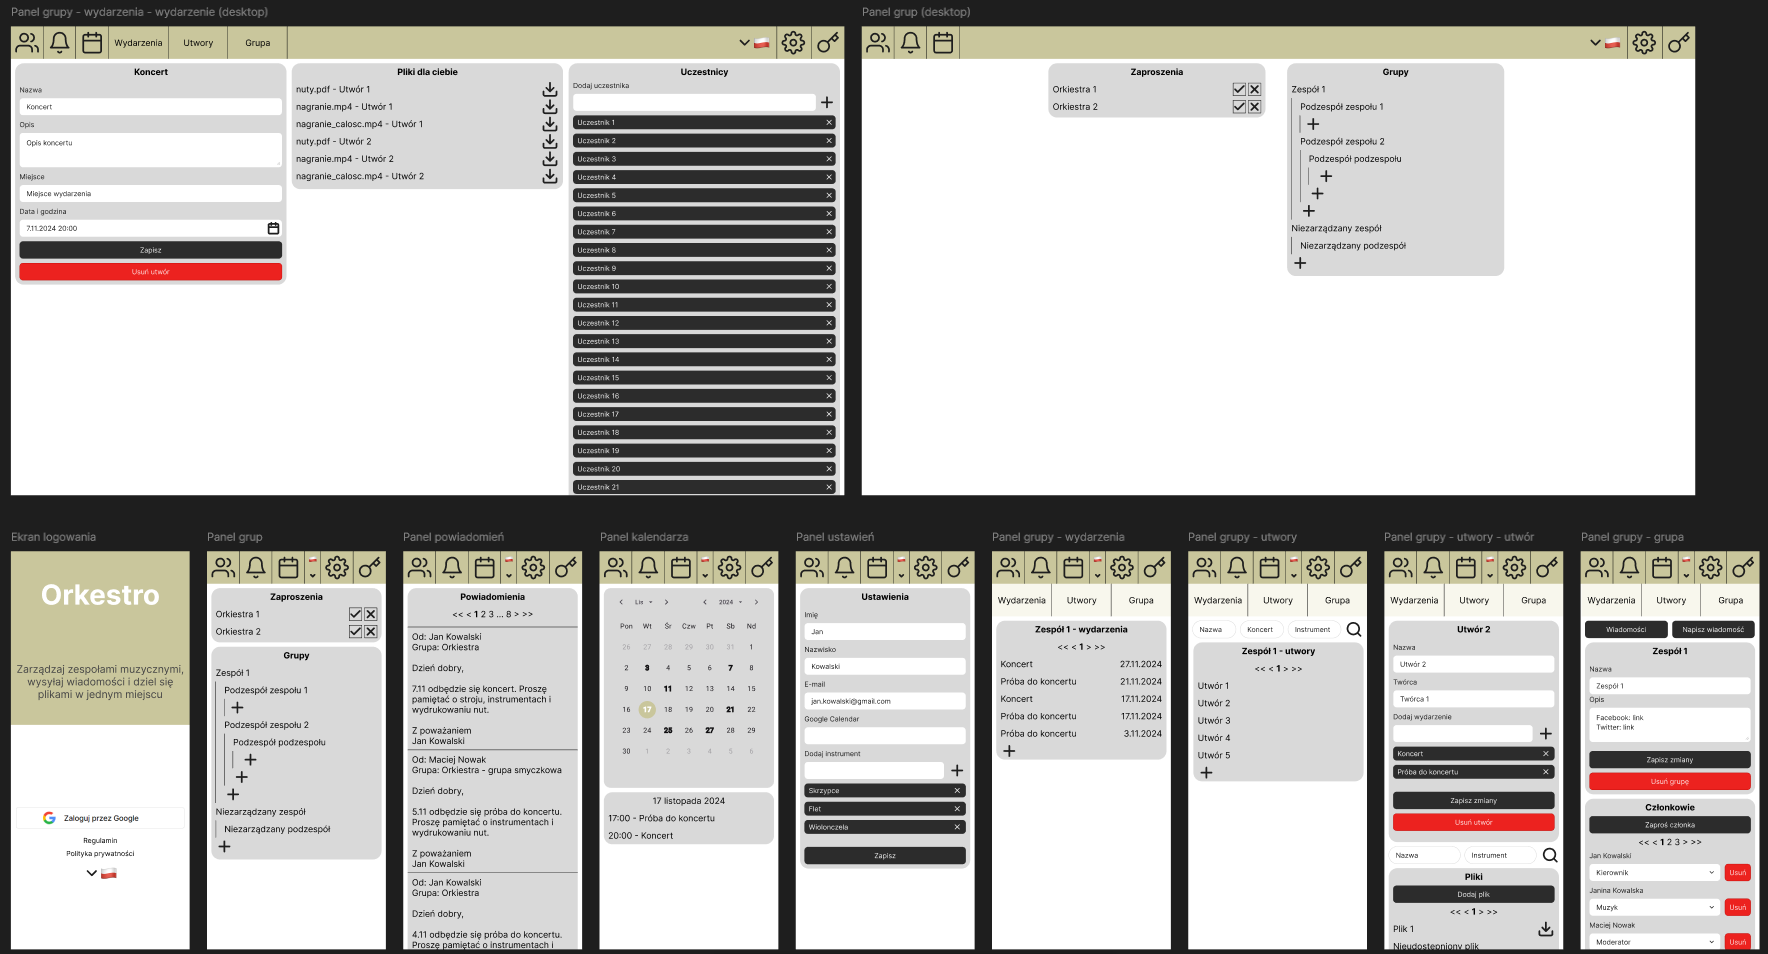
\includegraphics[width=0.95\linewidth]{images/makieta.png}
    \caption{Makiety najważniejszych ekranów aplikacji}
\end{figure}

\subsection{Styl wykonanej aplikacji}

Szata graficzna faktycznie wykonanej aplikacji:

\begin{figure} [H]
    \centering
    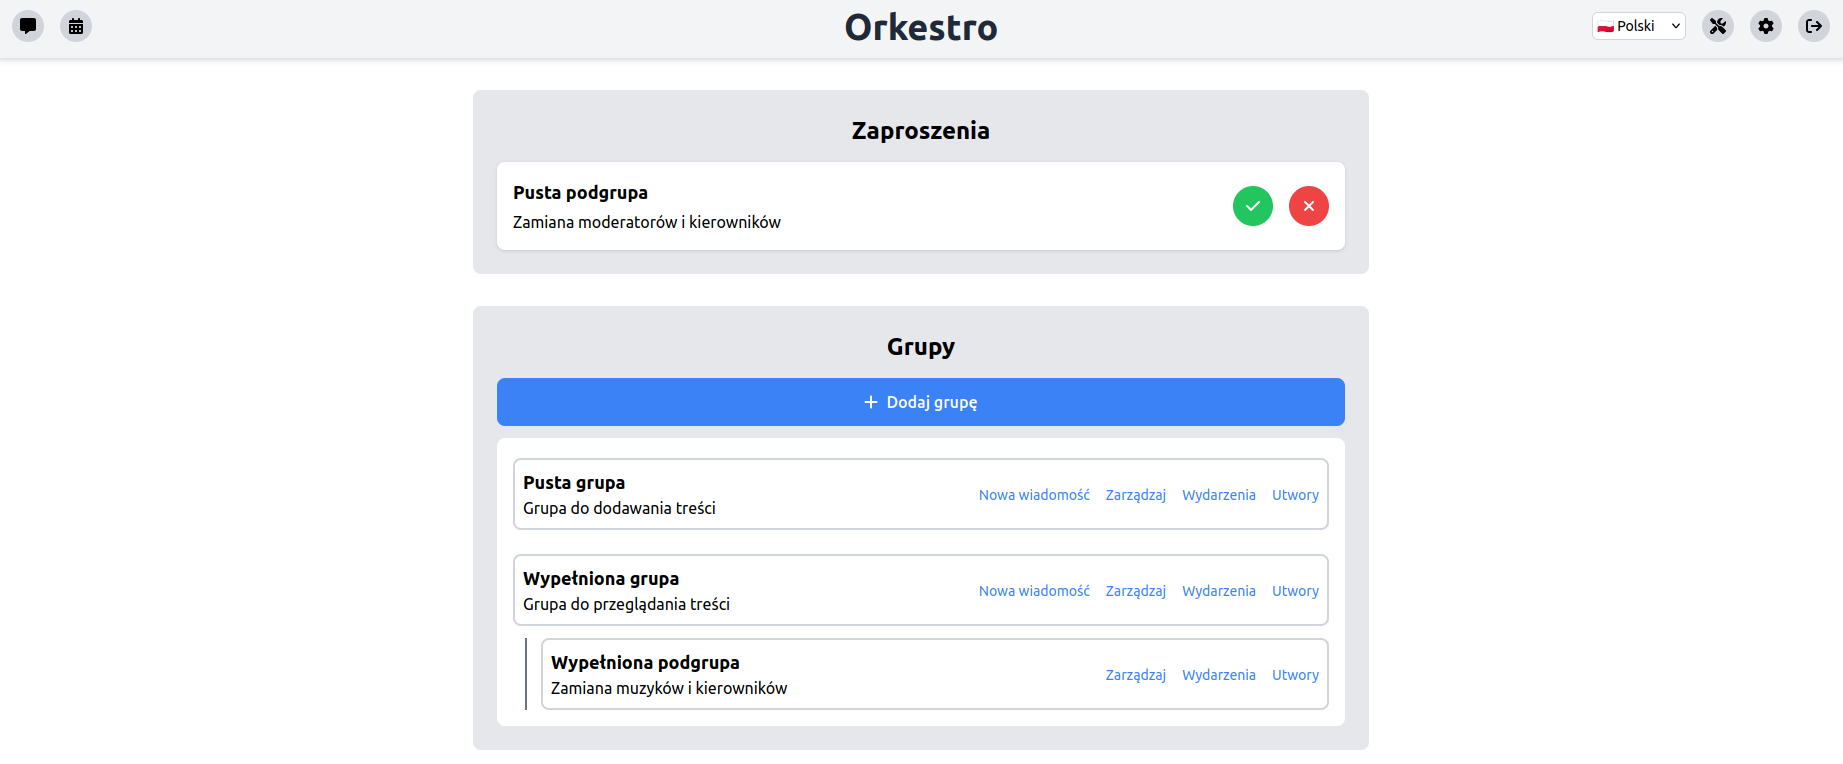
\includegraphics[width=0.95\linewidth]{images/aplikacja.png}
    \caption{Styl wykonanej aplikacji}
\end{figure}

Główne zmiany, które zaszły w interakcjach z aplikacją względem wstępnego projektu:
\begin{itemize}
    \item wybór sekcji po wybraniu grupy zmieniono na jej natychmiastowy wybór wraz z grupą
    \item komponenty są rozłożone w pionie zamiast w poziomie
    \item podgrupę tworzy się w panelu zarządzania grupą
    \item można wyszukiwać więcej zasobów, niż ujęto w wymaganiach; dostępne jest jedno pole do wyszukiwania po wszystkich kryteriach
    \item niektóre informacje nieistotne dla muzyków są widoczne tylko w formularzu do edycji
    \item w informacjach o wydarzeniu zamiast listy plików jest lista utworów, a po kliknięciu któregoś jest dostępna jego lista plików
    \item przeniesiono wysyłanie i odbieranie wiadomości wewnątrz grupy - wysyłanie jest dostępne natychmiast w panelu z grupami, a przeglądanie - w zbiorczym panelu wiadomości, przy użyciu wyszukiwania
    \item informacje o użytkowniku są w większości pobierane z konta Google - modyfikować można Google Calendar i listę instrumentów
\end{itemize}

\section{Specyfikacja testów}

\subsection{Obsługa błędów}

Serwer weryfikuje spójność danych przesyłanych w zapytaniach z modelem danych i resztą informacji w systemie oraz uprawnienia użytkowników do wykonania danej akcji. Jeżeli wykryje jakąś nieprawidłowość, zwraca odpowiedni kod błędu: 400 Bad Request dla niepoprawnych zapytań, 401 Unauthorized dla niezalogowanych użytkowników, 403 Forbidden dla niewystarczających uprawnień, 404 Not Found dla nieistniejących zasobów. Przy wyłączonym backendzie może również wystąpić błąd 502 Bad Gateway.

\subsection{Testowanie serwera}

Do backendu zostały napisane testy jednostkowe. Sprawdzają one m.in. poprawność działania klas, reakcje na błędne dane czy brak uprawnień. Testy zostały napisane we frameworku \texttt{unittest}, a sprawdzanie stopnia pokrycia odbywa się poprzez \texttt{coverage.py}. Miary jakości testów:
\begin{itemize}
    \item liczba testów: 151
    \item odsetek przechodzących testów: 100\%
    \item pokrycie linii testami: 92\%
    \item pokrycie gałęzi testami: 89\%
\end{itemize}

\subsection{Testy systemowe}

Zgodność systemu z wymaganiami można sprawdzić następującym zestawem testów (część wymagań ma elementy, których ocena jest z natury subiektywna - w tych przypadkach przydatne jest weryfikacja ich spełnienia przez kilka osób):
\begin{itemize}
    \item Wymaganie B1 - do oceny na podstawie stopnia realizacji pozostałych wymagań.
    \item Wymagania U1-U18, S1-S29 - należy zweryfikować, czy w serwisie da się wykonać daną akcję jako użytkownik o danych uprawnieniach. Za scenariusze testowe można przyjąć przypadki użycia zdefiniowane w rozdziale 3.3. Modyfikacja i usuwanie danych dotyczy tworzonych zasobów, z pewnymi wyjątkami (usuwanie wiadomości i ich odbiorców, usuwanie/degradacja siebie jako ostatniego kierownika grupy, usuwanie siebie jako ostatniej osoby z dostępem do pliku).
    \item Wymaganie U18, część o dodawaniu języków - powinna być dostępna procedura dodawania języków, ponadto należy ocenić jej pracochłonność.
    \item Wymagania U19, S30 - należy zweryfikować, czy system wspiera replikację bazy danych oraz funkcjonowanie dowolnej liczby kontenerów z Django REST API, do tego zasymulować obciążenie podane w wymaganiu i sprawdzić, czy serwer z wystarczająco dużymi zasobami będzie responsywny.
    \item Wymagania U20, S34, S35 - korzystając z poszczególnych systemów i przeglądarek, należy otwierać stronę internetową i sprawdzać, czy utracona została jakaś funkcjonalność.
    \item Wymagania U21, S36 - należy upewnić się, że akcji wymienionych w przypadkach użycia nie da się wykonać jako użytkownik o niższych uprawnieniach niż podane (poprzez aplikację lub API). W przypadku większości danych dostępnych w ramach grupy hierarchia uprawnień jest następująca: kierownik - moderator - członek grupy - użytkownik niebędący członkiem grupy - osoba niezalogowana do serwisu. Ponadto użytkownik nie powinien mieć dostępu do nieadresowanych do siebie plików, wiadomości i zaproszeń oraz modyfikować danych nie swojego konta.
    \item Wymaganie S31 - do określenia na podstawie tej dokumentacji.
    \item Wymagania S32, S33 - należy ocenić, jak komfortowe jest korzystanie ze strony internetowej na obu typach urządzeń.
    \item Wymaganie S37 - należy zweryfikować zgodność systemu z przepisami RODO.
    \item Wymaganie S38 - należy zweryfikować, czy system wspiera serwowanie aplikacji przez HTTPS.
    \item Wymaganie S39 - należy ocenić, jak dobrze system jest chroniony przed włamaniami.
    
\end{itemize}

\section{Wirtualizacja/konteneryzacja}

System może być wdrażany na maszynach wirtualnych zapewnionych przez Azure. Korzystamy z Dockera do tworzenia i uruchamiania kontenerów z komponentami systemu.

\section{Bezpieczeństwo}

W celu zapewnienia bezpieczeństwa (przed włamaniami, nieuprawnionym dostępem do danych, utratą danych, ...) system jest wyposażony w następujące zabezpieczenia:
\begin{itemize}
    \item System wdrożony na chmurze Azure funkcjonuje w większości w sieci lokalnej - jedyną maszyną dostępną bezpośrednio z zewnątrz jest ta serwująca aplikację poprzez NGINX.
    \item System wdrożony na chmurze Azure ma skonfigurowanego firewalla - dla zewnętrznych maszyn dostępny jest tylko port SSH i ten, na którym serwowana jest aplikacja. Dalsze połączenia odbywają się poprzez reverse proxy.
    \item Dostęp do maszyn systemu wymaga posiadania kluczy SSH wygenerowanych przy jego wdrożeniu.
    \item Wrażliwe parametry takie jak hasło do bazy danych są przechowywane w pliku \texttt{.env}.
    \item Korzystanie z aplikacji wymaga logowania; odbywa się to poprzez konto Google, które jest bezpieczniejsze od implementacji loginu i hasła oraz umożliwia uwierzytelnianie wieloskładnikowe.
    \item Panel administratora jest zabezpieczony przed atakami CSRF.
    \item Backend jest napisany w Django, które posiada wbudowane mechanizmy bezpieczeństwa, m.in. ochrona przed SQL injection.
    \item System korzysta z tokenów JWT o ograniczonym czasie życia.
    \item Zaimplementowany jest system uprawnień - przed udzieleniem dostępu do zasobu sprawdzane jest, czy użytkownik ma prawo wykonać daną akcję.
    \item Dostęp do aplikacji odbywa się poprzez HTTPS/SSL.
    \item System umożliwia wykonanie zrzutu danych oraz odtworzenie systemu z zadaną kopią danych.
    \item System funkcjonuje zgodnie z przepisami RODO.
\end{itemize}

\section{Podręcznik użytkownika}

Instrukcja będzie przedstawiana z perspektywy kierownika grupy - użytkownicy o niższych uprawnieniach nie mogą edytować ani usuwać danych grupy, a muzycy nie mogą wysyłać wiadomości.

\subsection{Logowanie i strona główna}

Po wejściu na stronę ukaże się ekran logowania - można wykonać logowanie kontem Google, wybrać język aplikacji i przeczytać politykę prywatności:

\begin{figure} [H]
    \centering
    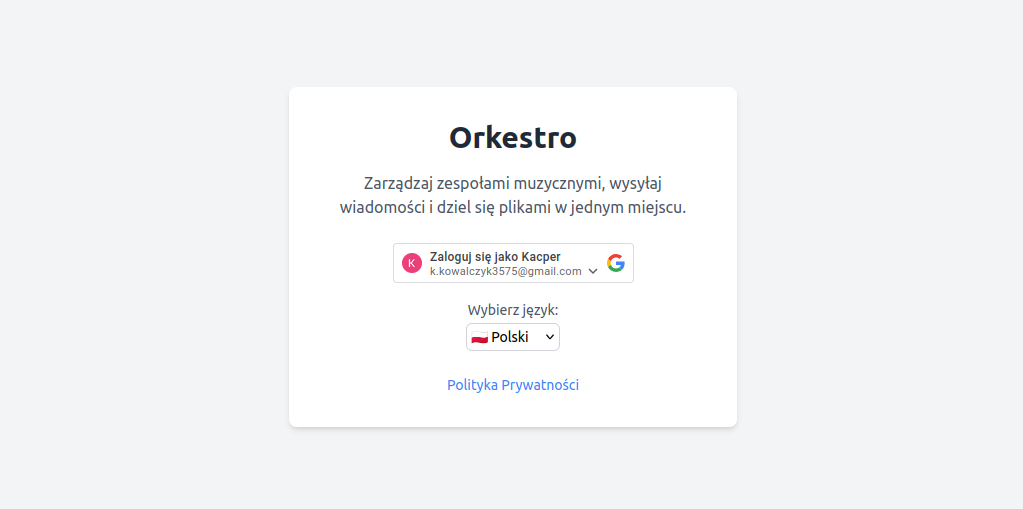
\includegraphics[width=0.95\linewidth]{images/instrukcja_login.png}
    \caption{Logowanie}
\end{figure}

Po wybraniu konta Google i zalogowaniu się do niego ukaże się główny ekran aplikacji:

\begin{figure} [H]
    \centering
    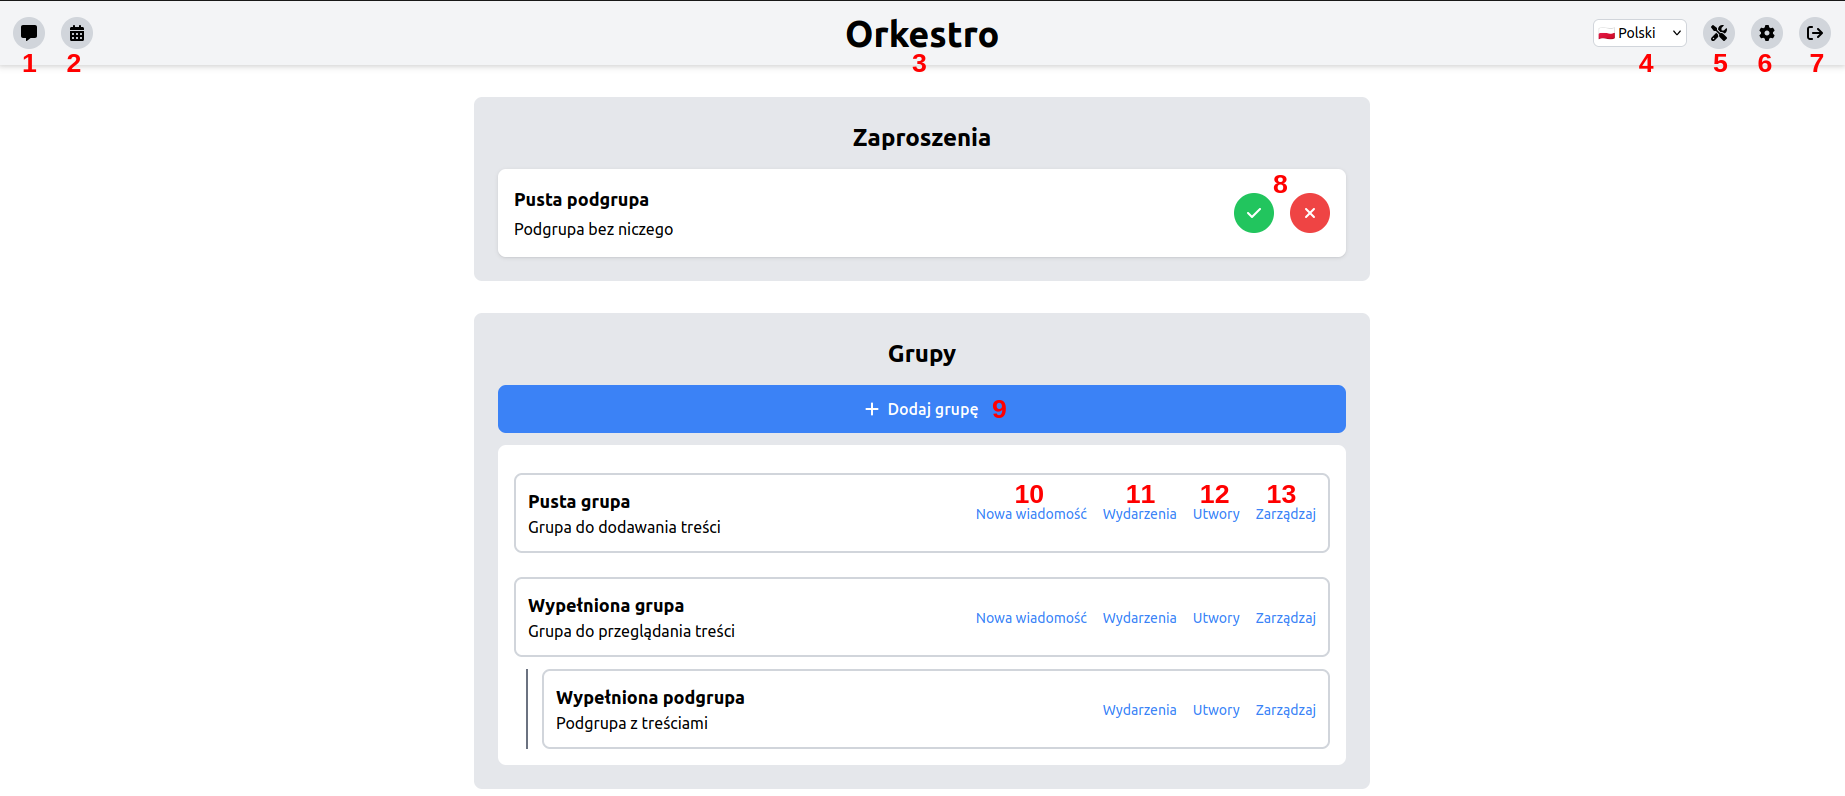
\includegraphics[width=0.95\linewidth]{images/instrukcja_grupy.png}
    \caption{Główny ekran}
\end{figure}

Można stąd przeglądać wiadomości (1), kalendarz wydarzeń (2), zmienić język (4), zmieniać ustawienia konta (6), wylogować się (7), przeglądać zaproszenia do grup, jeżeli istnieją i odpowiadać na nie (8), stworzyć własną grupę (9) lub przeglądać istniejące: napisać wiadomość (10), przeglądać wydarzenia (1), utwory z plikami (12) i dane grupy (13). Użytkownicy z uprawnieniami administratora mogą ponadto przechodzić do panelu administratora Django (5). Do tego panelu można wracać, klikając logo w górnej części ekranu (3).

\subsection{Panel ustawień}

W panelu ustawień można przeglądać dane konta i łączyć się z Google Calendar - po kliknięciu przycisku "Połącz" należy wybrać konto Google i udostępnić je aplikacji. Potem można aktualizować listę wydarzeń, gdy pojawią się nowe.

Widoczne są też instrumenty użytkownika. Można dodawać nowe, wybierając je z listy i zatwierdzając wybór, lub usuwać istniejące.

\begin{figure} [H]
    \centering
    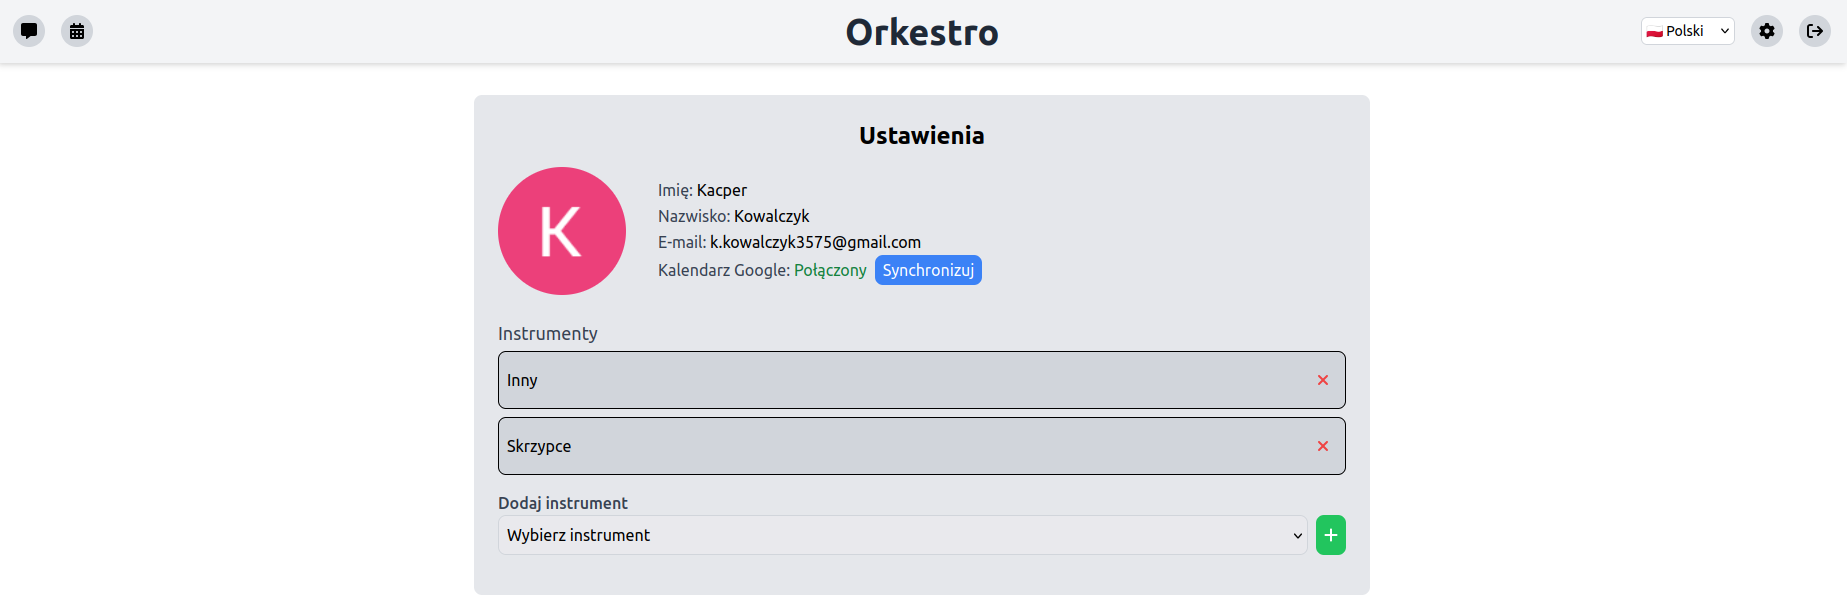
\includegraphics[width=0.95\linewidth]{images/instrukcja_ustawienia.png}
    \caption{Panel ustawień}
\end{figure}

\subsection{Panel administratora}

Django oferuje wbudowany panel administratora. Użytkownicy o odpowiednich uprawnieniach mogą z niego skorzystać, by przeglądać całość danych w bazie oraz dodawać, modyfikować i usuwać je bez ograniczeń narzucanych przez UI aplikacji. Panel jest dostępny tylko w języku angielskim - jest to zewnętrzny, dodatkowy komponent, który zintegrowaliśmy ze stroną.

\begin{figure} [H]
    \centering
    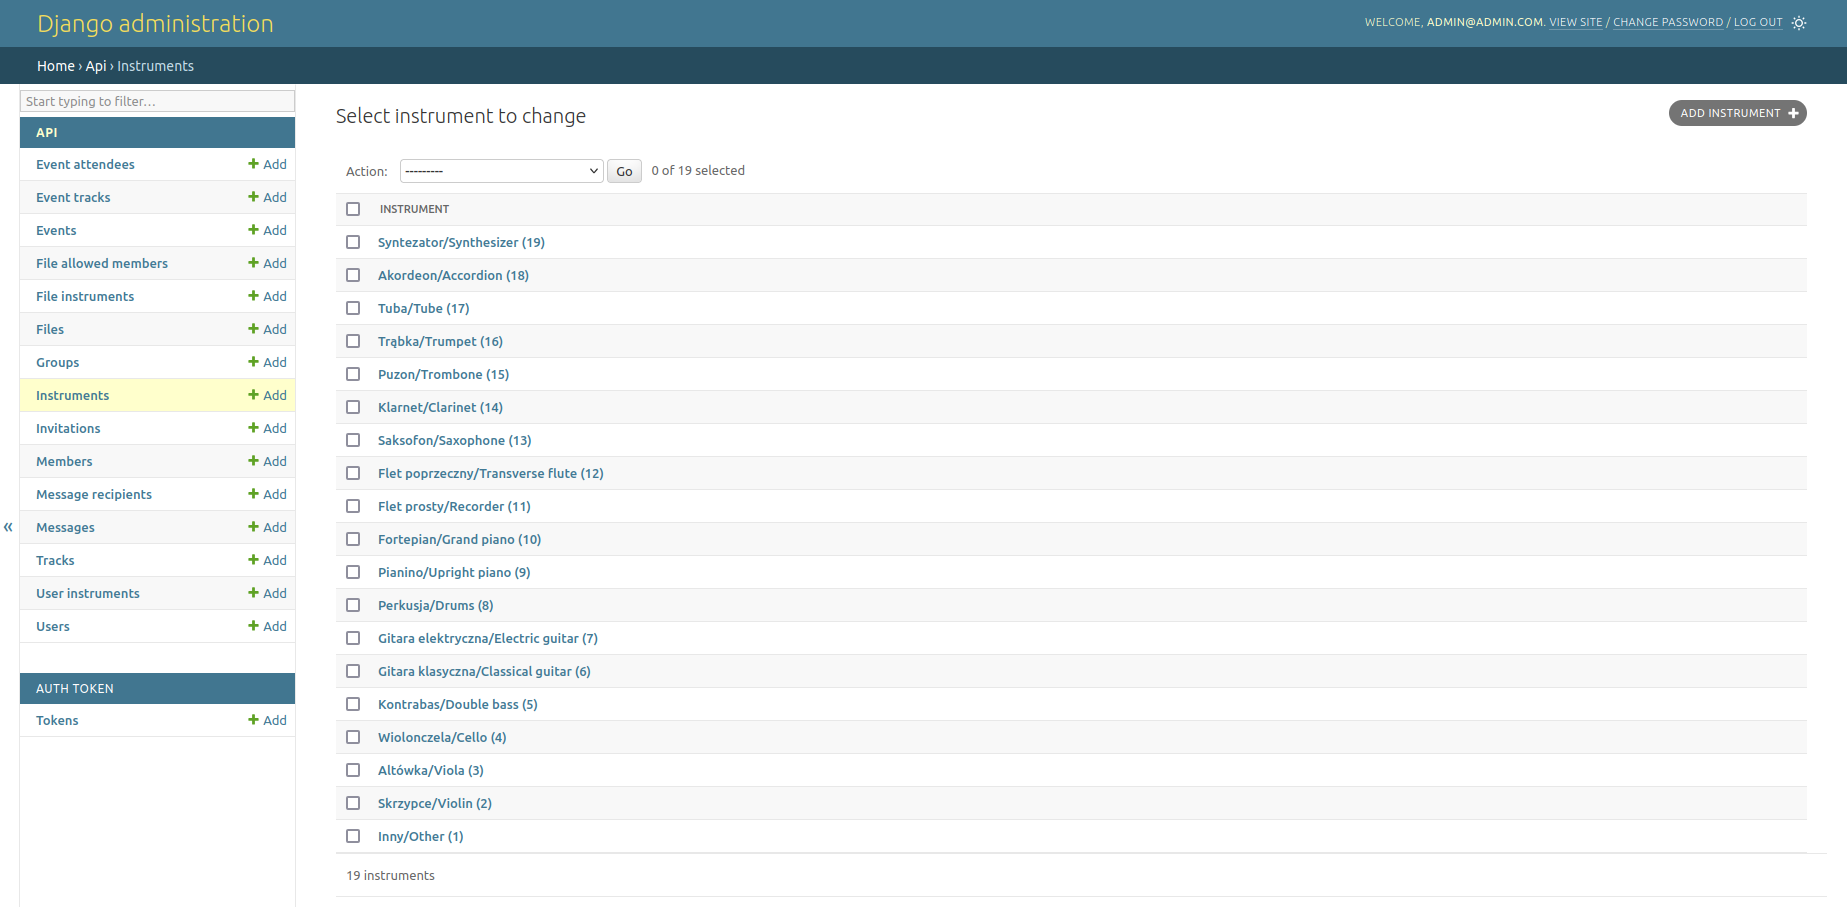
\includegraphics[width=0.95\linewidth]{images/instrukcja_admin.png}
    \caption{Panel administratora z otwartą zakładką z instrumentami}
\end{figure}

\subsection{Panel wiadomości}

W tym panelu można przeglądać wiadomości ze wszystkich grup. Aby wyświetlić treść którejś, należy ją kliknąć. Nieprzeczytane wiadomości podświetlają się na żółto. Oprócz ich treści podawany jest ich autor, grupa pochodzenia oraz data i godzina wysłania. Wiadomości są pogrupowane w strony, istnieje możliwość ich wyszukiwania po tytule, autorze i grupie pochodzenia.

\begin{figure} [H]
    \centering
    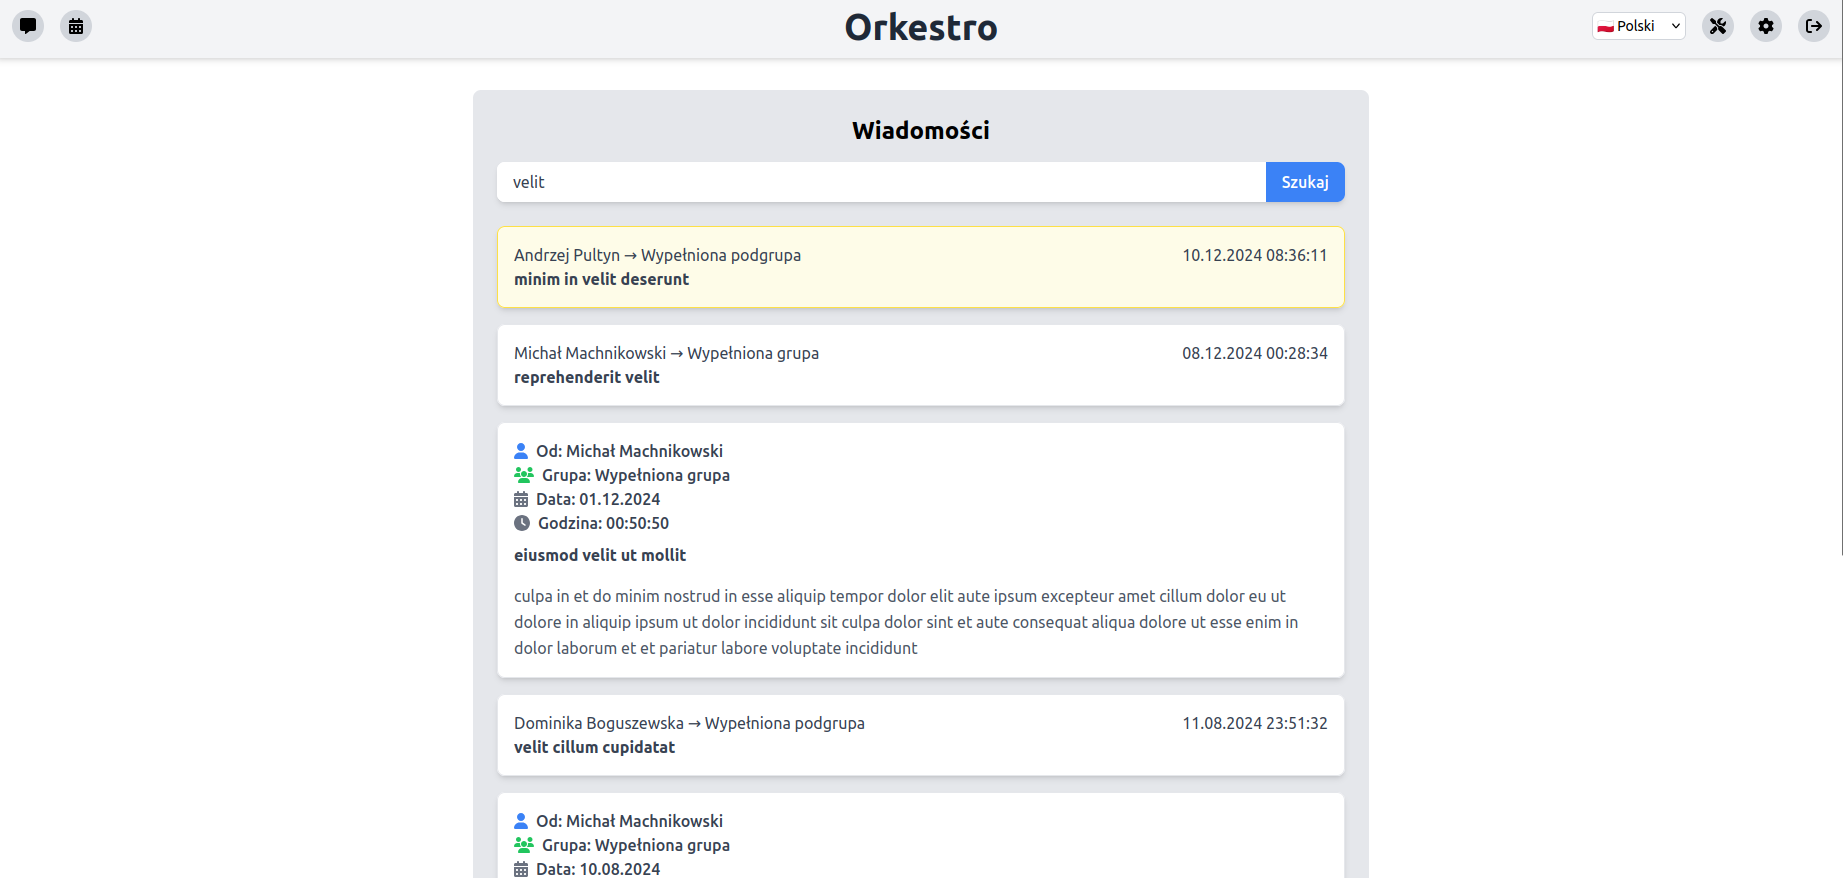
\includegraphics[width=0.95\linewidth]{images/instrukcja_wiadomosci.png}
    \caption{Panel wiadomości}
\end{figure}

\subsection{Kalendarz wydarzeń}

Tutaj można przeglądać wszystkie wydarzenia, których jest się uczestnikiem. Można przewijać miesiące i lata oraz cofać się do obecnego miesiąca. Po kliknięciu danego dnia w kalendarzu pojawiają się wydarzenia, które mają się wtedy odbyć - można je kliknąć, by przenieść się do informacji o tym wydarzeniu (przydatne, by szybko pobrać potrzebne na nim pliki, np. nuty).

\begin{figure} [H]
    \centering
    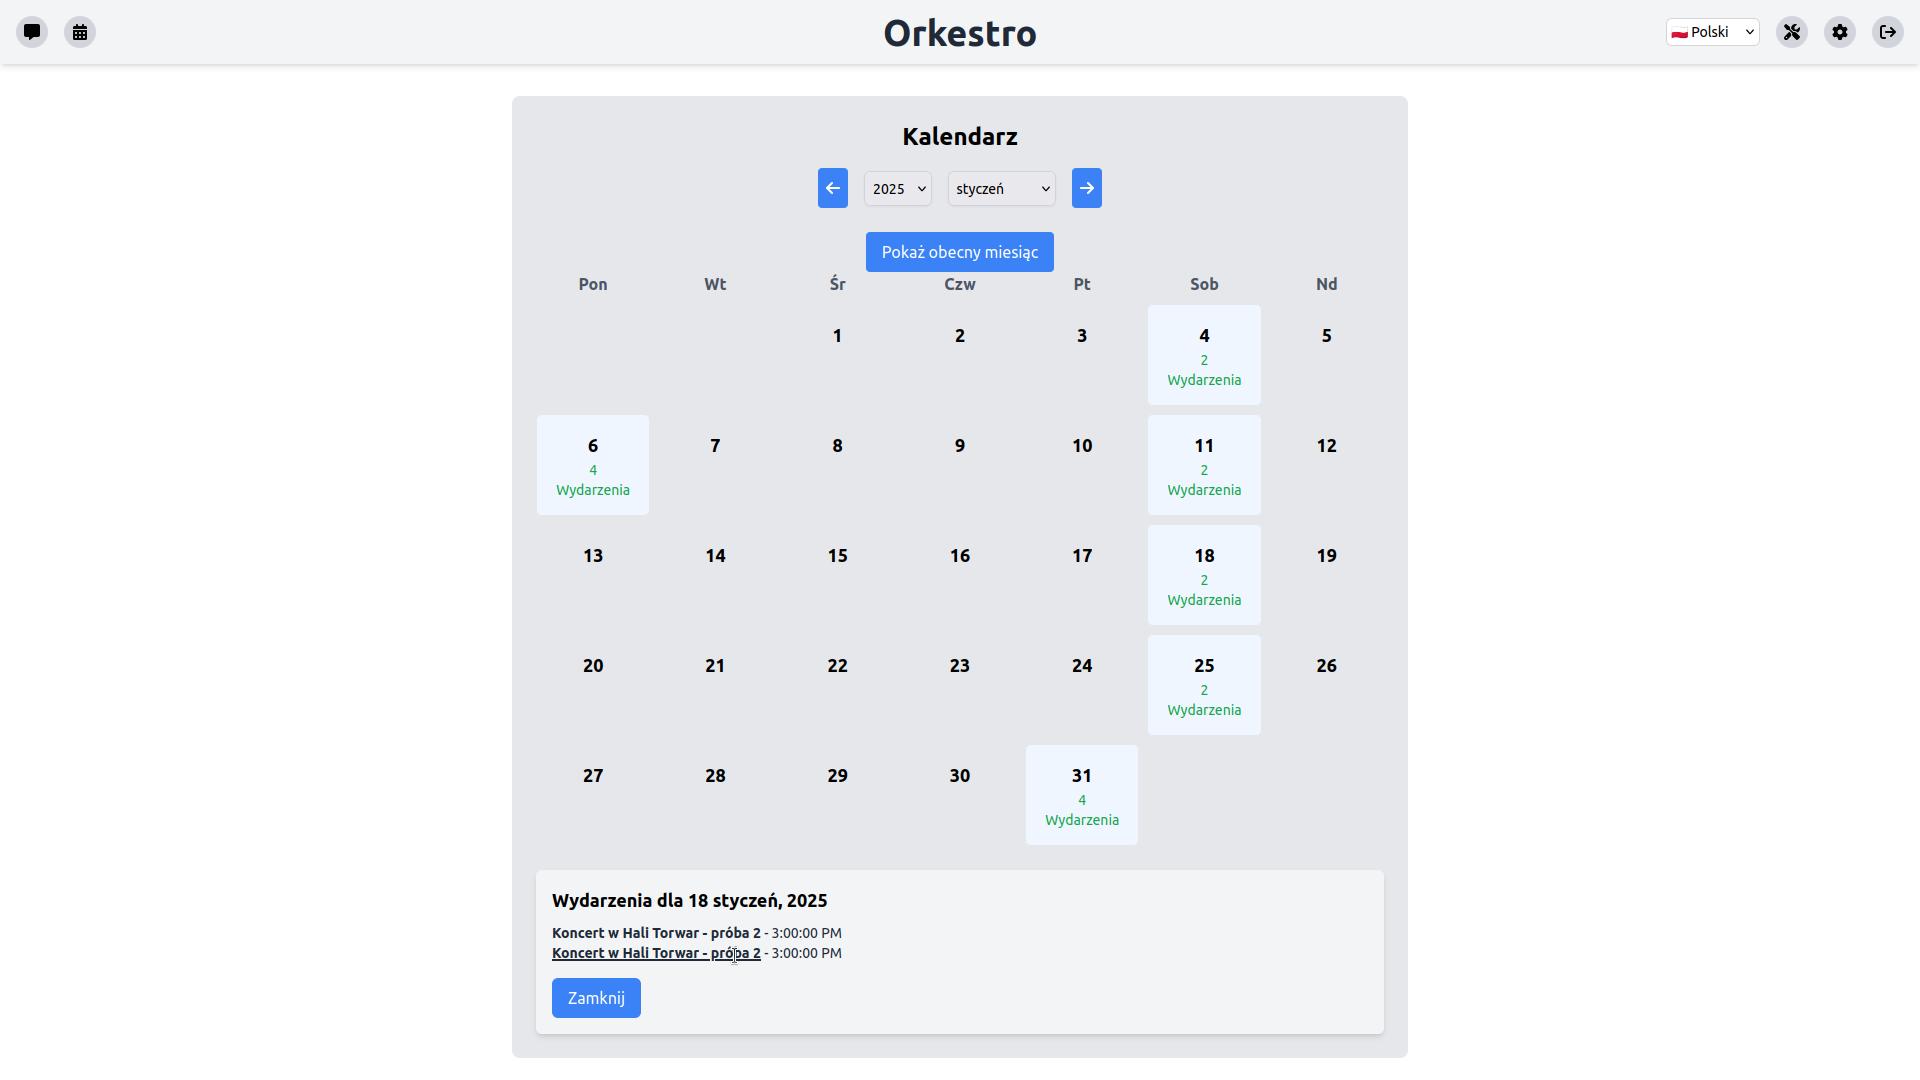
\includegraphics[width=0.95\linewidth]{images/instrukcja_kalendarz.png}
    \caption{Kalendarz wydarzeń}
\end{figure}

\subsection{Panel grupy}

Tutaj można przeglądać listę członków grupy (z możliwością wyszukiwania, filtrowania po uprawnieniach, zmieniania uprawnień i wyrzucania z grupy) i zapraszać nowych - trzeba znać adres e-mail zapraszanego użytkownika. Aby samemu opuścić grupę, należy skorzystać z przycisku nad listą (nie można być ostatnim kierownikiem). Nie można wyrzucać samego siebie lub zmieniać swoich uprawnień.

Jest możliwość edycji informacji o grupie i jej kasowania. Można też utworzyć podgrupę dla tej grupy. Pozostałe przyciski umożliwiają skorzystanie z reszty zakładek, które były dostępne w ogólnym panelu grup.

\begin{figure} [H]
    \centering
    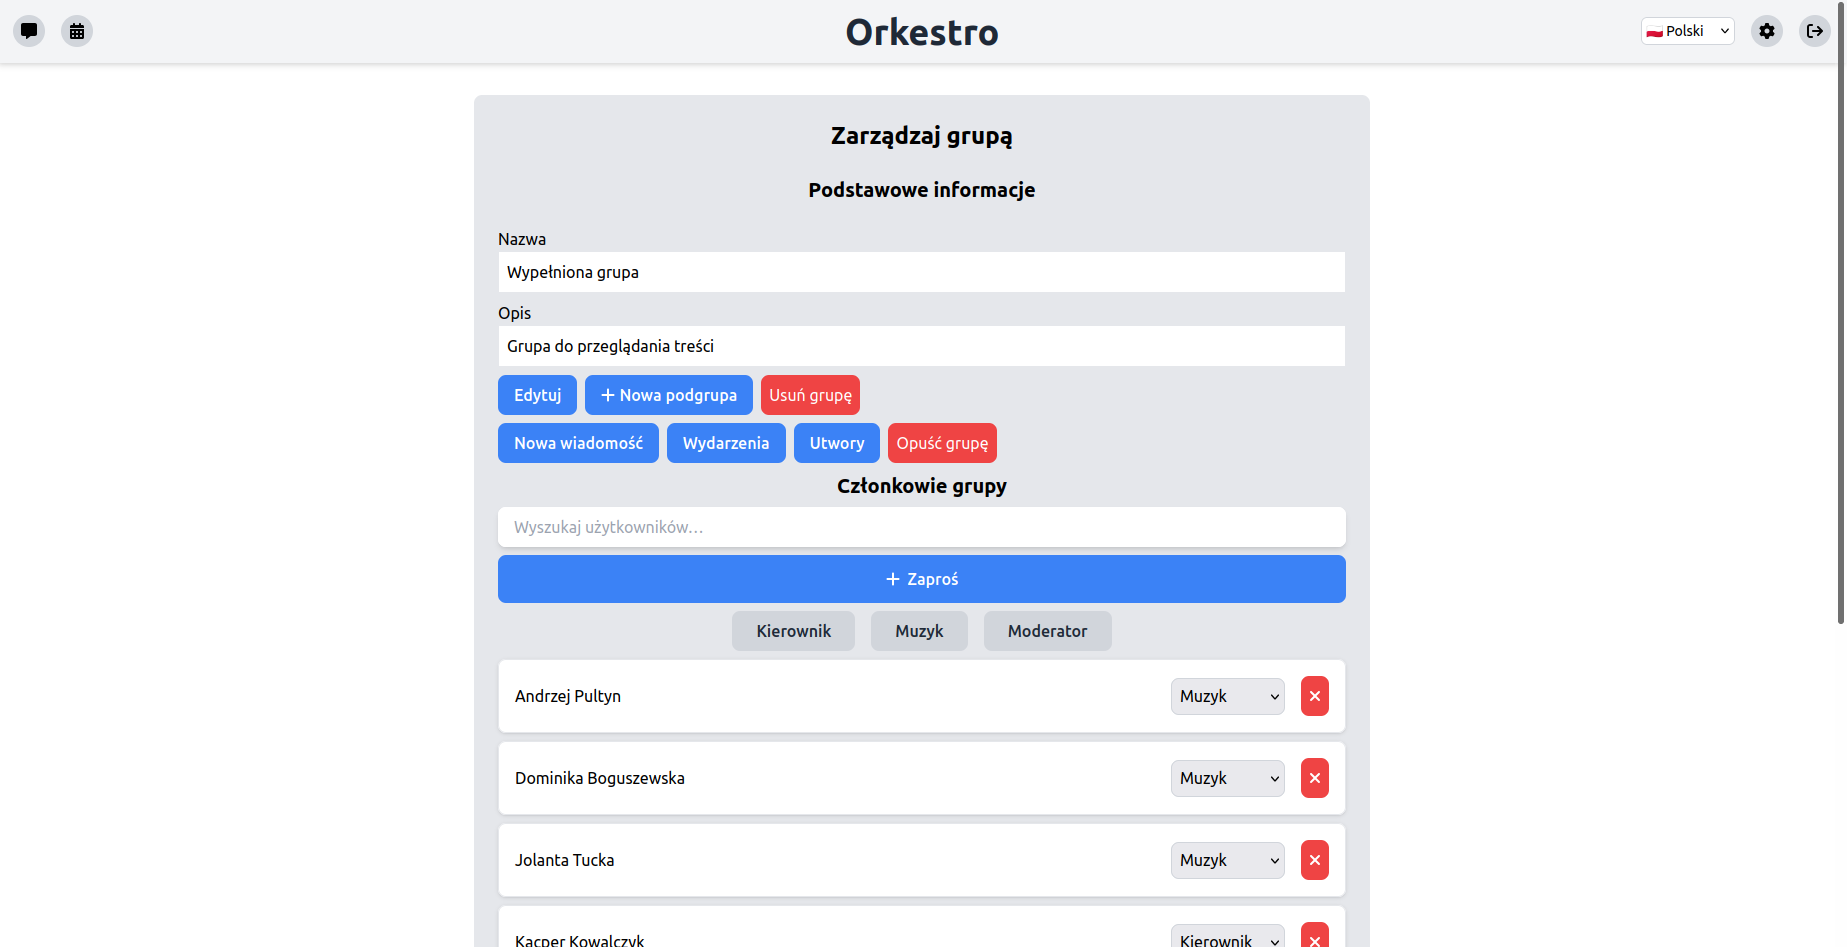
\includegraphics[width=0.95\linewidth]{images/instrukcja_grupa.png}
    \caption{Panel grupy}
\end{figure}

\subsection{Panel wydarzeń grupy}

Tutaj można przeglądać, dodawać, edytować i usuwać wydarzenia zdefiniowane dla danej grupy. Po wybraniu wydarzenia pokazują się szczegóły dla niego (data, godzina, miejsce odbywania się, opis z dodatkowymi informacjami) oraz lista granych na nim utworów - można je klikać, by się do nich przenosić. Dostępna jest wyszukiwarka dla wydarzeń filtrująca po nazwie, miejscu lub opisie.

Przy dodawaniu wydarzeń możliwość podpinania utworów jest niedostępna, ale można to zrobić, edytując nowo powstałe wydarzenie.

\begin{figure} [H]
    \centering
    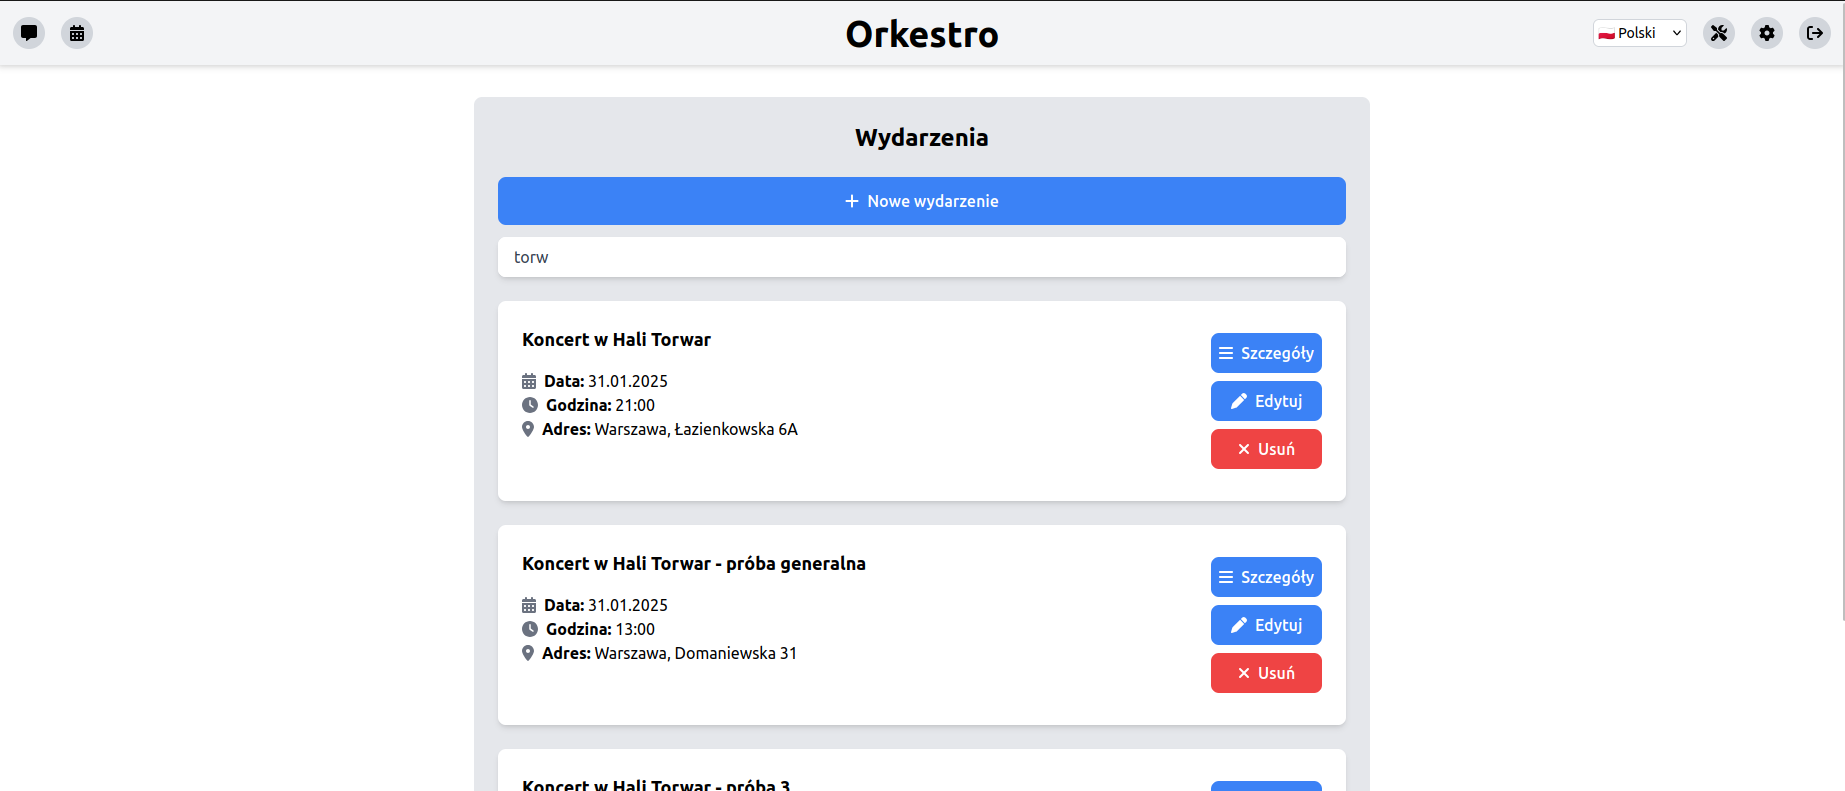
\includegraphics[width=0.95\linewidth]{images/instrukcja_wydarzenia.png}
    \caption{Panel wydarzeń}
\end{figure}

\begin{figure} [H]
    \centering
    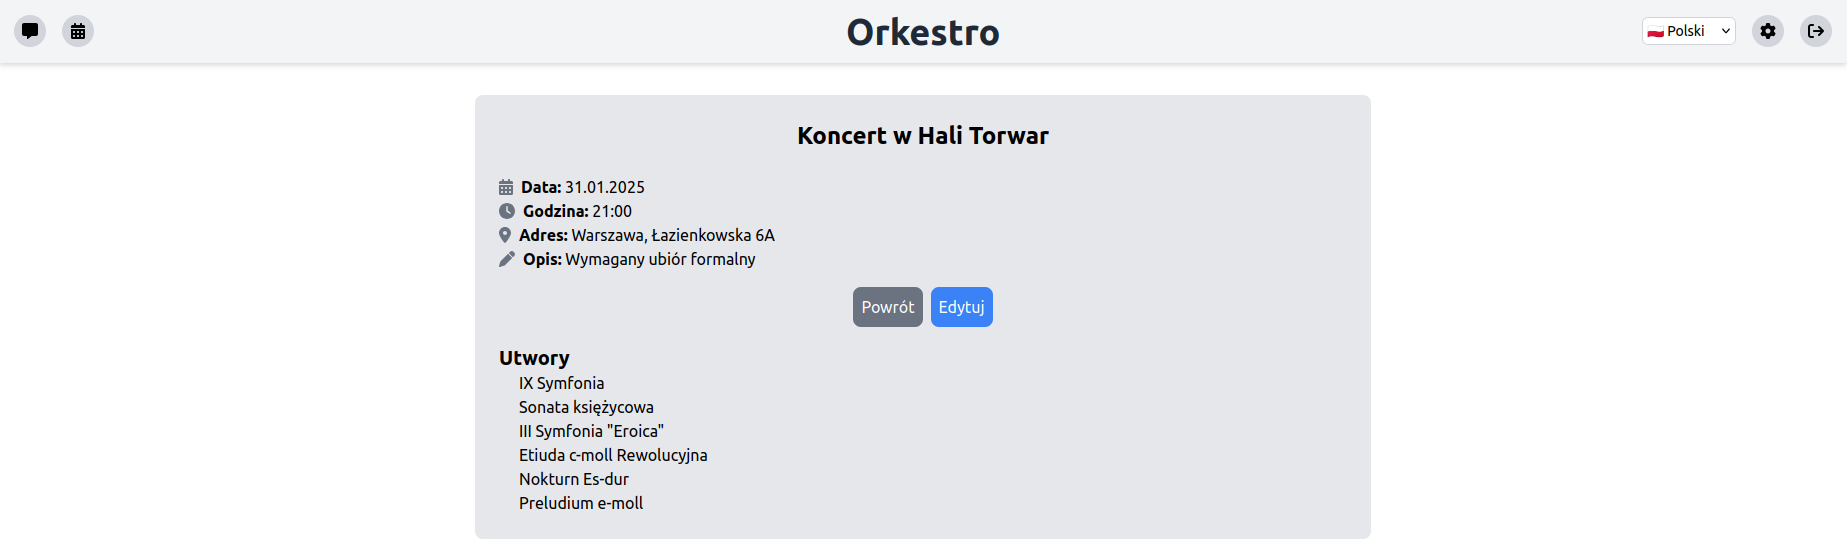
\includegraphics[width=0.95\linewidth]{images/instrukcja_wydarzenie.png}
    \caption{Panel wydarzeń - szczegóły o wydarzeniu}
\end{figure}

\subsection{Panel utworów}

Tutaj można przeglądać utwory, dodawać nowe i je usuwać. Jest możliwość wyszukiwania po nazwie, powiązanych wydarzeniach i instrumentach (same utwory nie są nimi oznaczone - wyszukiwanie odbywa się po instrumentach podpiętych plików).

\begin{figure} [H]
    \centering
    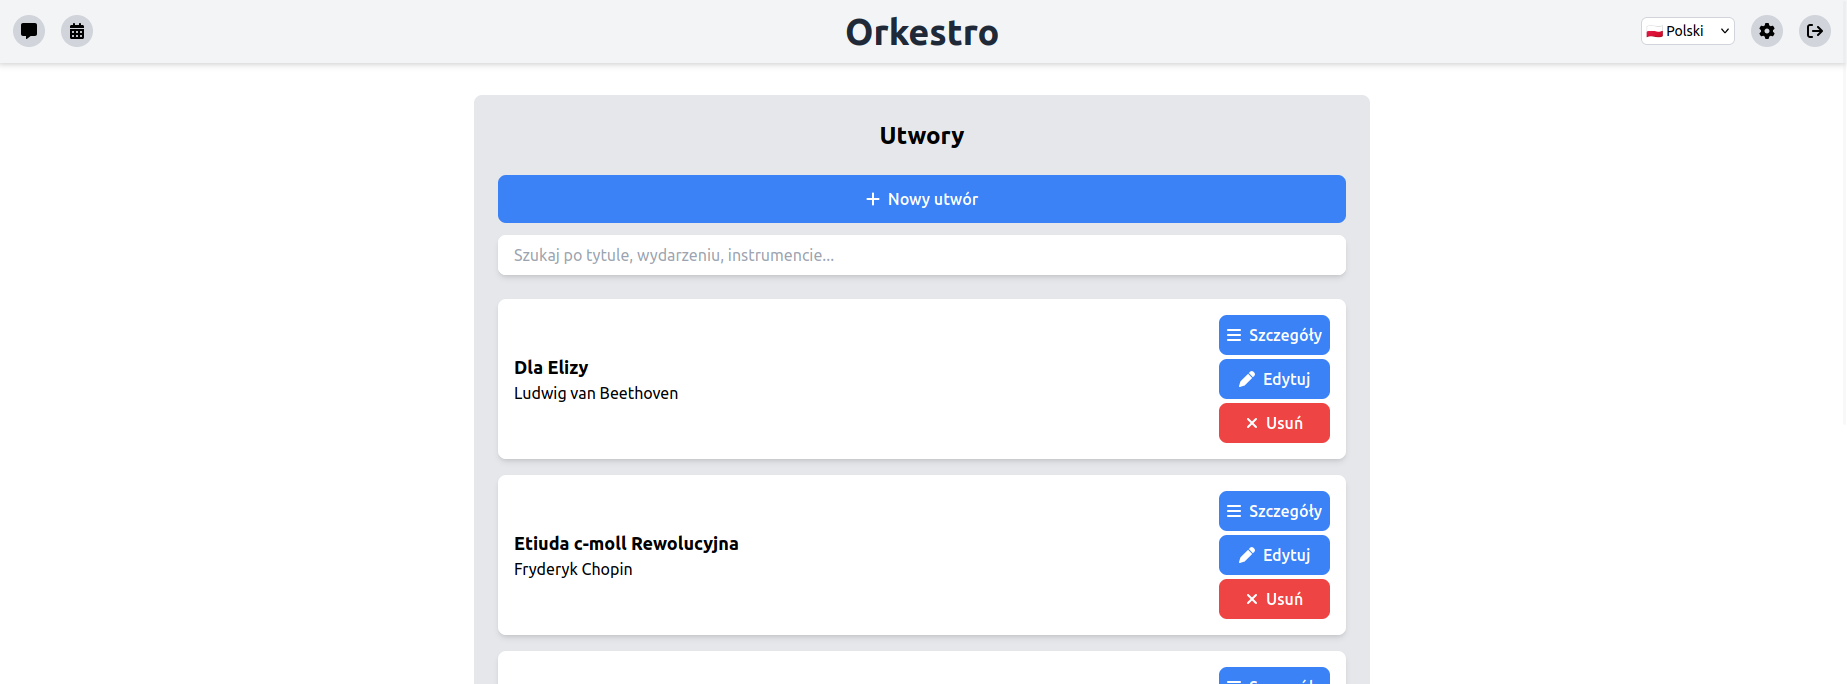
\includegraphics[width=0.95\linewidth]{images/instrukcja_utwory.png}
    \caption{Panel utworów}
\end{figure}

Po wybraniu utworu można przejrzeć podpięte pliki, które zostały udostępnione przeglądającemu (i je pobrać) oraz nadchodzące wydarzenia, z którymi związany jest utwór.

\begin{figure} [H]
    \centering
    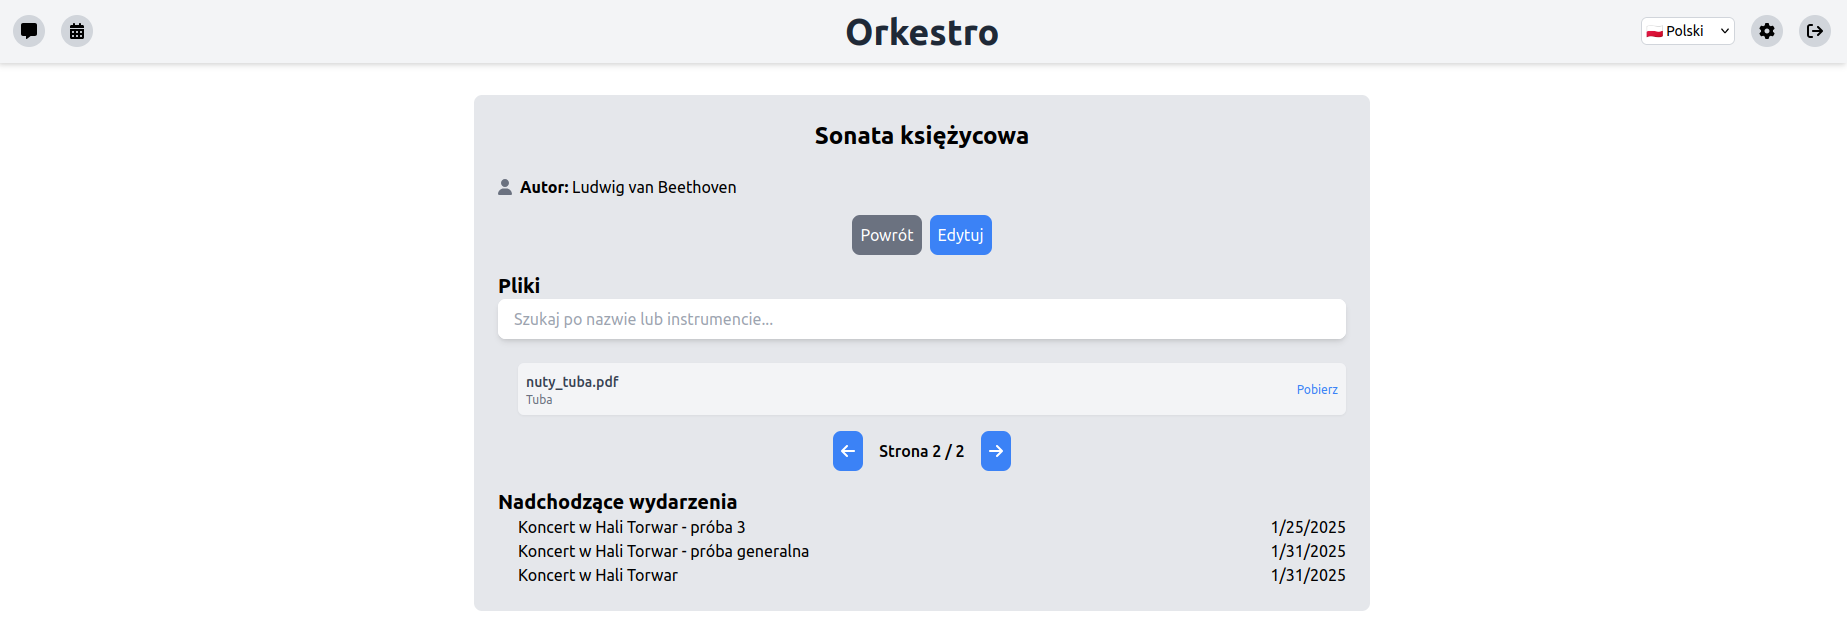
\includegraphics[width=0.95\linewidth]{images/instrukcja_utwor.png}
    \caption{Panel utworów - utwór}
\end{figure}

Pliki dodaje się (i usuwa) w formularzu do edycji utworu. Należy wgrać plik, wybrać członków grupy, którzy mają mieć do niego dostęp i wybrać podpięte instrumenty.

\begin{figure} [H]
    \centering
    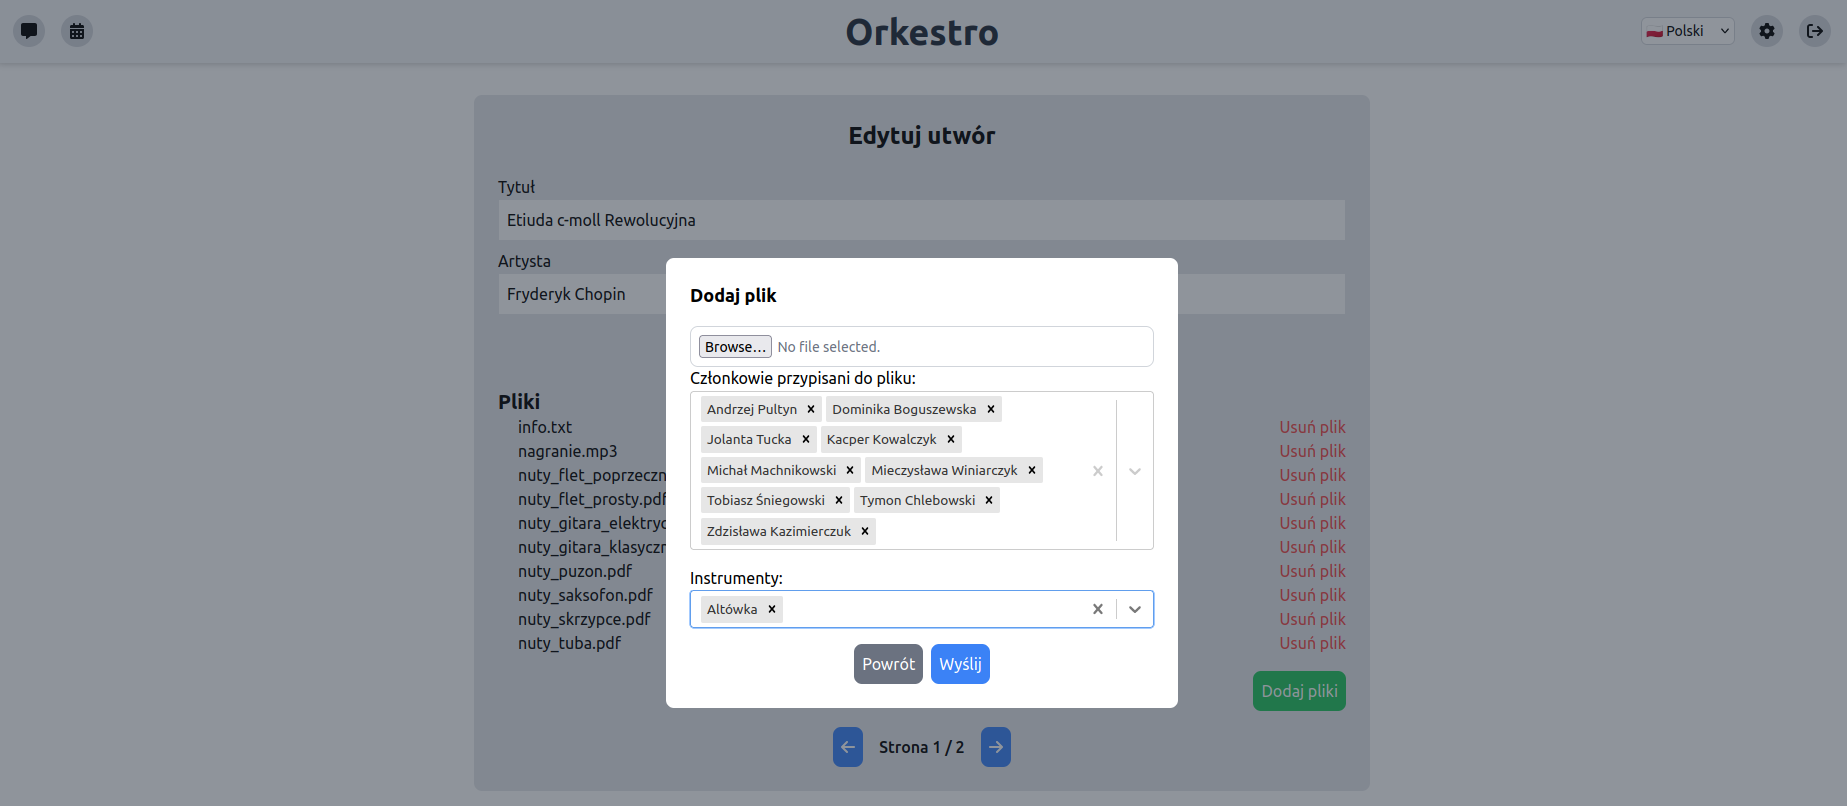
\includegraphics[width=0.95\linewidth]{images/instrukcja_plik.png}
    \caption{Panel utworów - utwór - dodawanie pliku}
\end{figure}

\subsection{Dodawanie wiadomości}

Tutaj moderatorzy i kierownicy mogą pisać wiadomości. Należy wybrać listę adresatów, wpisać tytuł i treść oraz wybrać, czy kopia wiadomości powinna być wysłana również na e-mail.

\begin{figure} [H]
    \centering
    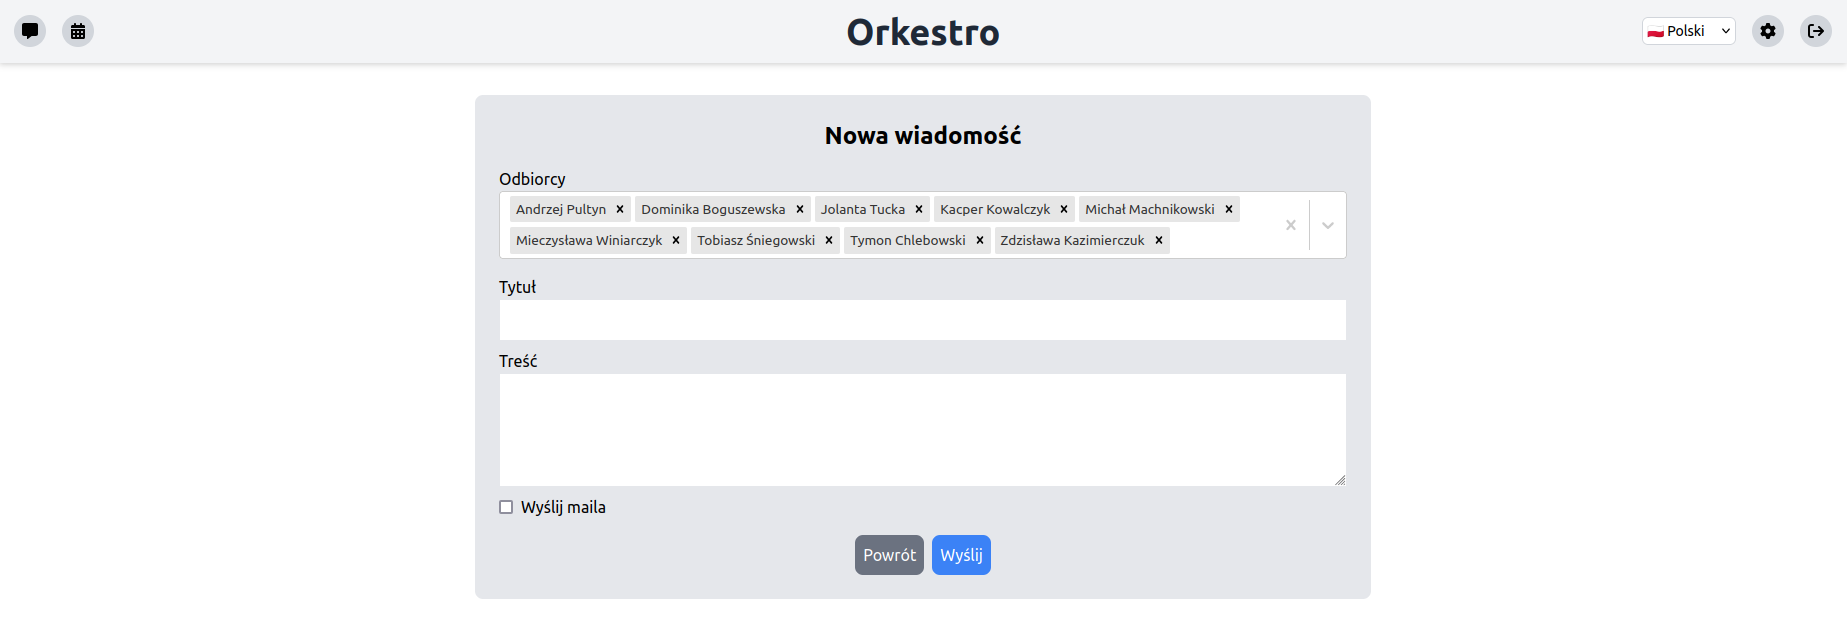
\includegraphics[width=0.95\linewidth]{images/instrukcja_wiadomosc.png}
    \caption{Panel dodawania wiadomości}
\end{figure}

\section{Podręcznik administratora}

\subsection{Czynności wstępne}

Należy sklonować repozytorium: \url{https://gitlab-stud.elka.pw.edu.pl/zgromadzeni/orkestro}

Do lokalnego uruchomienia potrzebny jest Docker, a wdrożenie na chmurę wymaga zainstalowania Azure CLI i zalogowania się tam (na koncie muszą znajdować się środki do opłacania maszyn). Komendy Dockera wymagają uprawnień administratora lub dodania użytkownika wykonującego komendy do grupy \texttt{docker}.

Potrzebne jest uzyskanie identyfikatora klienta interfejsu API Google (\url{https://console.developers.google.com/}) oraz jego sekretnego klucza. Należy w konfiguracji włączyć interfejs Google Calendar i dodać URI, na których będzie działać system (np. lokalnie: \texttt{http://localhost:5000}, przy wdrożeniu: \texttt{https://orkestro.ddns.net:5000}).

Do wysyłania e-maili potrzebne jest konto Google z wygenerowanym hasłem do aplikacji: \url{https://support.google.com/mail/answer/185833}

Dodatkowo do udostępnienia aplikacji innym użytkownikom potrzebne jest pozyskanie domeny (np. korzystając z DDNS) oraz certyfikatu dla niej - Google wymaga szyfrowania SSL dla aplikacji dostępnych z zewnątrz. Pliki \texttt{chain.pem}, \texttt{fullchain.pem} i \texttt{privkey.pem} należy umieścić w folderze \texttt{nginx}.

Należy utworzyć w katalogu głównym projektu plik \texttt{.env} z zawartością podaną w \texttt{readme} repozytorium. Znaczenie parametrów (zaznaczone na \textcolor{orange}{pomarańczowo} wymagają dostosowania, \textcolor{purple}{fioletowo} - dodatkowo, przy udostępnianiu aplikacji innym):
\begin{itemize}
    \item POSTGRES\_DB - nazwa bazy danych
    \item \textcolor{purple}{INCLUDE\_TEST\_DATA} - czy dodawać przykładowe dane (najlepiej wyłączyć przy wdrożeniu)
    \item POSTGRES\_MASTER\_USER, \textcolor{orange}{POSTGRES\_MASTER\_PASSWORD}, \textcolor{orange}{POSTGRES\_MASTER\_HOST}, POSTGRES\_MASTER\_PORT - parametry do łączenia się z bazą danych master (użytkownik, hasło, adres IP, port); jeżeli adres to localhost, należy wpisać adres prywatny typu \texttt{192.168.x.x}
    \item \textcolor{orange}{USE\_SLAVE}, POSTGRES\_SLAVE\_USER, \textcolor{orange}{POSTGRES\_SLAVE\_PASSWORD}, \textcolor{orange}{POSTGRES\_SLAVE\_HOST}, POSTGRES\_SLAVE\_PORT - parametry do bazy danych slave; jeżeli używana jest jedna baza, to parametry poza \texttt{USE\_SLAVE} są nieistotne
    \item \textcolor{orange}{DJANGO\_KEY} - dowolnie wybrany, tajny klucz do Django
    \item \textcolor{purple}{DJANGO\_DEBUG} - czy włączać tryb Django udostępniający dodatkowe informacje do debugowania (wyłączyć przy wdrożeniu)
    \item DJANGO\_WORKERS - iloma wątkami powinno dysponować Django REST API
    \item EMAIL\_HOST, EMAIL\_PORT, \textcolor{orange}{EMAIL\_USER}, \textcolor{orange}{EMAIL\_PASSWORD} - parametry do wysyłania e-maili, należy wpisać adres e-mail konta i jego 16-znakowe hasło aplikacji
    \item \textcolor{purple}{DOMAIN}, \textcolor{purple}{IP} - domena/publiczny adres IP maszyny, który powinno akceptować Django REST API
    \item \textcolor{orange}{BACKEND\_HOSTS} - lista adresów IP i portów oddzielana spacją, na których nasłuchują komponenty Django; tutaj również zamiast localhosta należy używać adresu prywatnego
    \item \textcolor{orange}{REACT\_APP\_GOOGLE\_CLIENT\_ID} - uzyskany identyfikator do API Google
    \item \textcolor{orange}{GOOGLE\_CLIENT\_SECRET} - sekretna wartość powyższego klienta
    \item \textcolor{purple}{USE\_HTTPS} - czy NGINX powinien szyfrować połączenia (włączyć przy wdrożeniu)
    \item BROWSER - przy rozwijaniu aplikacji umożliwia wybór przeglądarki, którą otwiera \texttt{npm start}
    
\end{itemize}

\subsection{Podstawowe uruchomienie}

W \texttt{readme} repozytorium znajdują się podstawowe komendy do uruchomienia aplikacji. W tym wariancie baza danych i NGINX znajdują się w kontenerach, a backend i frontend startują bez ich wykorzystania (NGINX przekierowuje na serwer frontendu zamiast serwować pliki statyczne). Umożliwia to szybsze uruchamianie aplikacji z nowo wprowadzonymi zmianami.

Aplikacja jest dostępna na porcie 5000. Oprócz głównej strony dostępny jest m.in. panel administratora (\texttt{...:5000/admin/}) oraz API (\texttt{...:5000/api/}).

Gotową aplikację lepiej jest uruchamiać, korzystając z poniższej sekcji.

\subsection{Uruchomienie lokalnie}

Przy tworzeniu obrazów należy skorzystać ze skryptów tworzących bazy danych: \texttt{cd deployment/deploy \&\& sudo ./setup\_master.sh} i, jeżeli używane są dwie bazy: \texttt{sudo ./setup\_slave.sh}. Są one również odpowiedzialne za automatyczną migrację danych Django do bazy (ten etap może kilkukrotnie zwrócić błąd przed uzyskaniem połączenia z bazą) oraz umożliwienie replikacji. Po tej konfiguracji można normalnie uruchamiać te kontenery za pomocą \texttt{docker compose}.

Oprócz tego trzeba uruchomić serwisy dla frontendu i backendu: \texttt{docker compose up orkestro-backend orkestro-frontend -d}. Jeżeli frontend będzie zgłaszał problemy z siecią, należy skasować wszsytkie kontenery aplikacji i ponownie je stworzyć (\texttt{docker compose down}, \texttt{docker compose up <serwisy> -d}).

Serwisami działającymi w gotowym systemie są \texttt{orkestro-db-master, orkestro-db-slave, orkestro-backend, orkestro-frontend}. Można je zatrzymywać (\texttt{docker compose stop <serwisy\_oddzielone\_spacja>}) i ponownie uruchamiać (\texttt{docker compose start <serwisy\_oddzielone\_spacja>}).

\subsection{Wdrożenie na chmurę Azure}

W folderze \texttt{deploy} znajdują się skrypty umożliwiające wdrożenie systemu na chmurę. Do wdrożenia potrzebny jest klucz SSH umieszczony w \texttt{\textasciitilde /.ssh/orkestro.pem[.pub]} - można go wygenerować skryptem \texttt{create\_keys.sh}.

Dostępne są dwie wersje skryptu automatyzującego utworzenie potrzebnych zasobów w Azure (m.in. maszyn wirtualnych) oraz przeniesienie tam kodu i innych potrzebnych plików. Jedna (\texttt{add\_resources\_dev.sh}) kopiuje na chmurę całość projektu, w którym został uruchomiony skrypt (przy uruchamianiu warto tymczasowo wynieść stamtąd niepotrzebne foldery takie jak \texttt{node\_modules} czy \texttt{.git}) - umożliwia to testowe wdrożenie kodu, który nie znajduje się na gałęzi master. Druga klonuje repozytorium na maszynach i wysyła na nie pliki, których się tam nie przechowuje (\texttt{.env}, pliki certyfikatów, klucz SSH) - do jej użycia potrzebny jest jednak token dostępu GitLaba.

Skrypty te korzystają z plików konfiguracyjnych, które definiują m.in. liczbę maszyn wirtualnych, ich adresy IP oraz konfigurację firewalla. W folderze \texttt{deployment/configs} znajdują się przykładowe pliki dla jednej i czterech maszyn, odpowiadające im pliki .env oraz przykładowy plik konfiguracyjny, którym można dodać piątą maszynę do istniejącej grupy zasobów.

Wdrożenie odbywa się poprzez uruchomienie części wspólnej skryptów i jednego z wariantów pozostałej części, z plikiem konfiguracyjnym jako argumentem (i tokenem do Gitlaba, jeżeli potrzebny), np: 

\texttt{./create\_group.sh configs/four\_machines.sh \&\& ./add\_resources\_dev.sh configs/four\_machines.sh}

\texttt{./create\_group.sh configs/four\_machines.sh \&\& ./add\_resources.sh configs/four\_machines.sh <nazwa\_tokena> <wartosc\_tokena>}

Po wykonaniu zostanie podana gotowa do przeklejenia komenda do połączenia się z maszyną oraz adres IP, pod którym będzie dostępna aplikacja (trzeba podpiąć do niego domenę z certyfikatem, by działało logowanie Google). Z zewnątrz dostępna jest tylko jedna maszyna - do pozostałych trzeba wykonać jeszcze jedno połączenie SSH wewnątrz sieci prywatnej. Należy połączyć się z każdą maszyną i wdrożyć na nich planowane komponenty - robi się to tak samo, jak zostało to opisane w poprzedniej sekcji.

Skrypt \texttt{add\_resources(\_dev).sh} można wykonać ponownie na tej samej grupie, by dodać kolejne podsieci czy maszyny wirtualne - wystarczy zmodyfikować plik konfiguracyjny.

\subsection{Zarządzanie użytkownikami i uprawnieniami}

Zarządzanie użytkownikami i uprawnieniami (jak i inne czynności administracyjne) wykonuje się poprzez panel administratora. Aby uzyskać do niego dostęp, należy dodać pierwszego superużytkownika na którymkolwiek backendowym kontenerze: (\texttt{docker exec -it orkestro-backend python3 manage.py createsuperuser}). Program poprosi o adres e-mail i hasło. Tego konta można użyć do zalogowania się do panelu. Kolejne można dodawać tą samą komendą lub poprzez panel administratora, dodając ręcznie użytkowników i ustawiając im hasło. Można też nadawać istniejącym uprawnienia pracownika i/lub superużytkownika.

Zarządzanie użytkownikami i uprawnieniami w kontekście grup muzycznych wykonują kierownicy poprzez aplikację, ale panel administratora również umożliwia modyfikację danych w tabeli z członkami grup.

\subsection{Zarządzanie zasobami systemu}

Przed wykonaniem czynności modyfikujących strukturę systemu warto tymczasowo wyłączyć dostęp do aplikacji, zatrzymując kontener z frontendem, a przy czynnościach modyfikujących plik \texttt{.env} zapisywać zmiany również w pliku przechowywanym na maszynie administratora - może być przydatny jako backup.

Aby dodać kolejny kontener z backendem, należy stworzyć go na wybranej maszynie, a na maszynie z frontendem dodać w pliku \texttt{.env} prywatny adres IP i port nowego kontenera do \texttt{DJANGO\_HOSTS}. Następnie należy ponownie zbudować usługę z frontendem:

\texttt{docker compose down orkestro-frontend --rmi all ; docker compose up orkestro-frontend}

Usuwanie kontenera wykonuje się odwrotnie: skasowanie kontenera, usunięcie adresu z \texttt{.env}, ponowne zbudowanie frontendu.

Analogicznie wygląda procedura dodawania bazy danych slave: dodanie kontenera, wpisanie danych do łączenia z bazą (\texttt{POSTGRES\_SLAVE\_USER, POSTGRES\_SLAVE\_PASSWORD, POSTGRES\_SLAVE\_HOST, POSTGRES\ \_SLAVE\_PORT}) do pliku \texttt{.env} na każdej maszynie z uruchomionym backendem i ponowne zbudowanie tych usług:

\texttt{docker compose down orkestro-backend --rmi all ; docker compose up orkestro-backend}

Usunięcie takiej bazy wymaga usunięcia kontenera, przepisania danych do łączenia z bazą master na pola dla bazy slave w \texttt{.env} i ponownego zbudowania backendów.

\subsection{Aktualizacja oprogramowania}

System jest uruchamiany na kontenerach, co uniezależnia go od wersji oprogramowania występującego na maszynach (poza samym Dockerem). Wersje obrazów i zależności wewnątrz kontenerów są zapisane w plikach \texttt{Dockerfile}, \texttt{frontend/package.json}, \texttt{backend/requirements.txt} - w razie potrzeby można je zmodyfikować i ponownie zbudować odpowiednie serwisy:

\texttt{docker compose down <serwisy> --rmi all \&\& docker compose up <serwisy> -d}

Aby zaktualizować kod poszczególnych komponentów, należy pobrać zmiany (np. poprzez \texttt{git pull}), jeżeli trzeba - zaktualizować plik \texttt{.env}, po czym ponownie zbudować odpowiednie serwisy powyższą komendą.  

\subsection{Dodawanie języka}
Dodanie nowego języka wymaga następujących kroków:
\begin{itemize}
    \item w bazie danych: utworzyć nową kolumnę w tabeli \texttt{instruments} i wypełnić ją tłumaczeniami, zaktualizować plik SQL z definicją tabel i opcjonalnie z danymi testowymi
    \item we frontendzie: dodać nowy język do ogólnych plików frontendowych zajmujących się tłumaczeniem (\texttt{LanguageContext.tsx}, \texttt{i18n.js}), dodać same tłumaczenia w \texttt{locales}
    \item we frontendzie: dodać obsługę nowego języka w plikach mających do czynienia z danymi instrumentów lub wymagających dostosowania pisowni
\end{itemize}

\subsection{Kopia zapasowa i odtwarzanie systemu}

Backupów wymagają następujące dane:
\begin{itemize}
    \item kod
    \item plik \texttt{.env}
    \item pliki .pem  wykorzystywane do szyfrowania połączenia
    \item plik z konfiguracją maszyn w chmurze i klucz SSH wykorzystywany do łączenia się z nimi (jeżeli wykorzystywana chmura; przy odtwarzaniu systemu od zera klucz jest niepotrzebny, ale warto zabezpieczyć się przed jego zgubieniem)
    \item stan bazy danych master.
\end{itemize}

Pierwsze cztery pozycje są plikami dostępnymi z komputera administratora - wystarczy je  zarchiwizować. W celu wykonania backupu bazy danych należy wykonać w kontenerze kopię i przenieść ją do systemu plików - zakładając, że nazwa użytkownika do bazy danych i samej bazy to \texttt{myuser} i \texttt{orkestrodb}:

\texttt{docker exec -it orkestro-db-master /bin/sh -c "PGUSER=myuser pg\_dump -Fc orkestrodb > db.sql" \&\& docker cp orkestro-db-master:db.sql .}

Tak otrzymany plik można pobrać poprzez \texttt{scp} na maszynę z frontendem, a potem na komputer administratora. 

Przy odtwarzaniu systemu po utracie danych należy umieścić kopie plików na swoim miejscu i ponownie wykonać wdrożenie. Przy odtwarzaniu bazy danych master należy (po wykonaniu skryptu instalacyjnego) wysłać plik z kopią na odpowiednią maszynę, użyć go w kontenerze i ponownie wykonać migrację Django:

\texttt{docker cp db.sql orkestro-db-master:/ \&\& docker exec -it orkestro-db-master /bin/sh -c "export PGUSER=myuser ; dropdb orkestrodb ; createdb orkestrodb ; pg\_restore -d orkestrodb db.sql" \&\& docker compose up orkestro-backend-migrate}

Baza slave, jeżeli istnieje, samodzielnie pobierze odpowiednie dane.

\section{Podsumowanie}

Realizację projektu możemy uznać za udaną - zrealizowaliśmy na czas wszystkie wymagania klienta. Osiągnięcie celu ułatwiła kompozycja zespołu, która pozwoliła na efektywną współpracę, a umiejętności poszczególnych członków pokrywały dziedzinę projektu. W czasie pracy nad projektem dbaliśmy o jego jakość - pisaliśmy testy do kodu z analizą jego pokrycia, wzajemnie kontrolowaliśmy jakość dodawanego kodu i śledziliśmy spełnianie wymagań klienta. Przeprowadzaliśmy też refaktoring niektórych części projektu, gdy okazywało się, że można je napisać lepiej.

Przeszkodą w osiągnięciu celu było stosunkowo późne rozpoczęcie prac nad implementacją systemu, co skutkowało brakami w zakresie na etapach pośrednich projektu - w tym semestrze oprócz kolokwiów było do zrealizowania ponadprzeciętnie dużo różnych projektów zespołowych, co zmniejszało motywację do zajmowania się kolejnym, a rozproszenie odpowiedzialności opóźniło dodanie pierwszych funkcji do aplikacji.

Aplikacja ma pole do dalszego rozwoju - można w niej dodać np. śledzenie obecności na wydarzeniach (próbach do koncertów), automatyczne wyszukiwanie utworów, które mogłaby wykonywać dana grupa muzyków (na podstawie instrumentów, na których potrafią grać), obsadzanie poszczególnych głosów dla utworów granych na wydarzeniach czy obsługę dodatkowych języków.

Wizytówka projektu:

\begin{figure} [H]
    \centering
    
\includegraphics[width=0.95\linewidth]{images/wizytowka.png}
    \caption{Wizytówka}
\end{figure}


\section{Bibliografia}

\begin{enumerate}
    \item Materiały dydaktyczne do przedmiotu PZSP2, Politechnika Warszawska, 2024, Dostępne w Internecie dla uczestników kursu: \url{https://leon.pw.edu.pl/course/view.php?id=82}
    \item Przewodnik po Scrumie, Scrum Guides, 2020 [dostęp listopad 2020], Dostępny w Internecie: \url{https://scrumguides.org/docs/scrumguide/v2020/2020-Scrum-Guide-Polish.pdf}
    \item Django Documentation, Django Software Foundation, 2025 [dostęp 17 stycznia 2025], Dostępny w Internecie: \url{https://readthedocs.org/projects/django/downloads/pdf/5.0.x/}
\end{enumerate}

\section*{Zatwierdzam dokumentację}

\begin{flushright}
    \vspace{0.5cm}
    \rule{10cm}{0.2mm} \\
    Data i podpis Mentora
\end{flushright}

\end{document}
